\documentclass[12pt,a4paper]{report}

% ─────────────────────────────────────────
%  Encoding & Language
% ─────────────────────────────────────────
\usepackage[utf8]{inputenc}
\usepackage[T1]{fontenc}
\usepackage[english]{babel}

% ─────────────────────────────────────────
%  Page Layout
% ─────────────────────────────────────────
\usepackage[top=2.5cm, bottom=2.5cm, left=3cm, right=2.5cm]{geometry}

% ─────────────────────────────────────────
%  Typography
% ─────────────────────────────────────────
\usepackage{lmodern}
\usepackage{microtype}
\usepackage{setspace}
\onehalfspacing

% ─────────────────────────────────────────
%  Graphics & Colors
% ─────────────────────────────────────────
\usepackage{graphicx}
\graphicspath{{image/}{./}}
\usepackage[table,dvipsnames]{xcolor}
\definecolor{ibmblue}{RGB}{0,62,135}
\definecolor{snowblue}{RGB}{41,182,246}
\definecolor{lightgray}{RGB}{245,245,245}
\definecolor{darkgray}{RGB}{80,80,80}
\definecolor{accentblue}{RGB}{0,114,198}

% ─────────────────────────────────────────
%  Tables
% ─────────────────────────────────────────
\usepackage{array}
\usepackage{tabularx}
\usepackage{longtable}
\usepackage{multirow}
\usepackage{booktabs}
\usepackage{colortbl}

% ─────────────────────────────────────────
%  Figures & Floats
% ─────────────────────────────────────────
\usepackage{float}
\usepackage{caption}
\usepackage{subcaption}
\captionsetup{font=small, labelfont=bf, labelsep=period}

% ─────────────────────────────────────────
%  Lists
% ─────────────────────────────────────────
\usepackage{enumitem}
\setlist[itemize]{noitemsep, topsep=4pt}
\setlist[enumerate]{noitemsep, topsep=4pt}

% ─────────────────────────────────────────
%  Math
% ─────────────────────────────────────────
\usepackage{amsmath}
\usepackage{amssymb}

% ─────────────────────────────────────────
%  Code Highlighting
% ─────────────────────────────────────────
\usepackage{listings}
\lstset{
  basicstyle=\ttfamily\small,
  backgroundcolor=\color{lightgray},
  keywordstyle=\color{ibmblue}\bfseries,
  commentstyle=\color{darkgray}\itshape,
  stringstyle=\color{snowblue},
  breaklines=true,
  frame=single,
  rulecolor=\color{accentblue},
  numbers=left,
  numberstyle=\tiny\color{darkgray},
  captionpos=b,
  showstringspaces=false,
}

% listings has no built-in YAML language; define a minimal one so that
% GitHub Actions workflow listings (Ch.4 and Appendix B) compile.
\lstdefinelanguage{yaml}{
  comment=[l]{\#},
  morestring=[b]',
  morestring=[b]",
  keywords={true,false,null,on,push,pull_request,jobs,steps,uses,with,run,needs,name,env,if,id},
}

% ─────────────────────────────────────────
%  Gantt Chart
% ─────────────────────────────────────────
\usepackage{pgfgantt}
\usepackage{pdflscape}

% ─────────────────────────────────────────
%  TikZ / Diagrams
% ─────────────────────────────────────────
\usepackage{tikz}
\usetikzlibrary{shapes.geometric, arrows.meta, positioning, fit, backgrounds}

% ─────────────────────────────────────────
%  Headers & Footers
% ─────────────────────────────────────────
\usepackage{fancyhdr}
\pagestyle{fancy}
\fancyhf{}
\fancyhead[L]{\small\color{darkgray}\leftmark}
\fancyhead[R]{\small\color{darkgray}\thepage}
\fancyfoot[C]{\small\color{darkgray}Snowflake Environment Alignment \& CI/CD Pipeline --- ARYZTA Data Platform}
\renewcommand{\headrulewidth}{0.5pt}
\renewcommand{\footrulewidth}{0.3pt}

% ─────────────────────────────────────────
%  Chapter / Section Title Formatting
% ─────────────────────────────────────────
\usepackage{titlesec}
\titleformat{\chapter}[display]
  {\normalfont\Large\bfseries\color{ibmblue}}
  {\chaptertitlename\ \thechapter}{12pt}{\huge\color{ibmblue}}
\titlespacing*{\chapter}{0pt}{-10pt}{30pt}

\titleformat{\section}
  {\normalfont\large\bfseries\color{accentblue}}
  {\thesection}{1em}{}
\titleformat{\subsection}
  {\normalfont\normalsize\bfseries\color{darkgray}}
  {\thesubsection}{1em}{}
\titleformat{\subsubsection}
  {\normalfont\normalsize\itshape\color{darkgray}}
  {\thesubsubsection}{1em}{}

% ─────────────────────────────────────────
%  Hyperlinks
% ─────────────────────────────────────────
\usepackage{hyperref}
\hypersetup{
    colorlinks=true,
    linkcolor=ibmblue,
    filecolor=accentblue,
    urlcolor=snowblue,
    citecolor=accentblue,
    pdftitle={Snowflake Environment Alignment and CI/CD Pipeline Implementation for ARYZTA Data Platform},
    pdfauthor={Mouad Moulay Rachid},
    pdfsubject={End-of-Studies Internship Report --- IBM CIC Morocco / Hakkoda},
    pdfkeywords={Snowflake, CI/CD, DataOps, DevOps, IBM, Hakkoda, ARYZTA, GitHub, Data Engineering}
}

% ─────────────────────────────────────────
%  Bibliography
% ─────────────────────────────────────────
\usepackage[numbers,sort&compress]{natbib}

% ─────────────────────────────────────────
%  Acronyms & Glossary
% ─────────────────────────────────────────
\usepackage[acronym,toc]{glossaries}
\makeglossaries
% ═══════════════════════════════════════════════════════════════
%  Glossary & Acronyms
% ═══════════════════════════════════════════════════════════════

% ── Acronyms ───────────────────────────────────────────────────
\newacronym{ci}{CI}{Continuous Integration}
\newacronym{cd}{CD}{Continuous Delivery}
\newacronym{cicd}{CI/CD}{Continuous Integration and Continuous Delivery}
\newacronym{dev}{DEV}{Development Environment}
\newacronym{uat}{UAT}{User Acceptance Testing Environment}
\newacronym{prod}{PROD}{Production Environment}
\newacronym{devops}{DevOps}{Development and Operations}
\newacronym{dataops}{DataOps}{Data Operations}
\newacronym{ibm}{IBM}{International Business Machines Corporation}
\newacronym{cic}{CIC}{Client Innovation Center}
\newacronym{pr}{PR}{Pull Request}
\newacronym{iac}{IaC}{Infrastructure as Code}
\newacronym{sql}{SQL}{Structured Query Language}
\newacronym{ddl}{DDL}{Data Definition Language}
\newacronym{dml}{DML}{Data Manipulation Language}
\newacronym{etl}{ETL}{Extract, Transform, Load}
\newacronym{api}{API}{Application Programming Interface}
\newacronym{yaml}{YAML}{YAML Ain't Markup Language}
\newacronym{json}{JSON}{JavaScript Object Notation}
\newacronym{vcs}{VCS}{Version Control System}
\newacronym{scrum}{SCRUM}{Software Control and Risk Updating Method}
\newacronym{bi}{BI}{Business Intelligence}
\newacronym{erp}{ERP}{Enterprise Resource Planning}
\newacronym{dbt}{dbt}{data build tool}
\newacronym{rbac}{RBAC}{Role-Based Access Control}
\newacronym{snow}{Snowflake}{Snowflake Cloud Data Platform}
\newacronym{gh}{GH}{GitHub}
\newacronym{sn}{ServiceNow}{ServiceNow IT Service Management Platform}


% ─────────────────────────────────────────
%  Utility
% ─────────────────────────────────────────
\usepackage{pifont}
\usepackage{mdframed}
\usepackage{tcolorbox}
\tcbuselibrary{skins,breakable}

% Callout box style
\tcbset{
  notebox/.style={
    colback=lightgray,
    colframe=accentblue,
    fonttitle=\bfseries,
    title={Note},
    breakable,
    before skip=10pt,
    after skip=10pt,
  }
}

% ─────────────────────────────────────────
%  Custom Commands
% ─────────────────────────────────────────
\newcommand{\HRule}{\rule{\linewidth}{0.5mm}}
\newcommand{\placeholder}[2]{%
  \begin{tcolorbox}[colback=lightgray, colframe=darkgray!50, title=\texttt{[FIGURE PLACEHOLDER]}, fonttitle=\small\itshape]
  \centering\color{darkgray}\textit{#1}\\[4pt]\small#2
  \end{tcolorbox}
}

% ═══════════════════════════════════════════════════════════════
\begin{document}
% ═══════════════════════════════════════════════════════════════

\pagenumbering{roman}

% ── Cover Page ─────────────────────────────────────────────────
% ═══════════════════════════════════════════════════════════════
%  Cover Page
% ═══════════════════════════════════════════════════════════════
\thispagestyle{empty}

\begin{center}

  % ── Institution and Company Logos ──────────────────────────
  \begin{minipage}{0.30\textwidth}
    \begin{flushleft}
      
\includegraphics[width=0.85\textwidth]{ensias.jpg}
      
    \end{flushleft}
  \end{minipage}
  \hfill
  \begin{minipage}{0.30\textwidth}
    \begin{center}
      
\includegraphics[width=0.55\textwidth]{IBM.png}
      
    \end{center}
  \end{minipage}
  \hfill


  \vspace{0.6cm}
  \rule{\linewidth}{0.6pt}\\[0.3cm]

  {\large\bfseries Université Mohammed V --- Rabat}\\[0.15cm]
  {\large\bfseries École Nationale Supérieure d'Informatique et d'Analyse des Systèmes}\\[0.1cm]
  {\normalsize Filière : \textbf{Business Intelligence \& Analytics (BI\&A)}}\\[0.3cm]

  \rule{\linewidth}{0.6pt}\\[0.6cm]

  {\LARGE\bfseries\color{ibmblue} End-of-Studies Internship Report}\\[0.4cm]

  \rule{0.65\linewidth}{0.8pt}\\[0.4cm]

  {\LARGE\bfseries Snowflake Environment Alignment and}\\[0.2cm]
  {\LARGE\bfseries CI/CD Pipeline Implementation}\\[0.25cm]
  {\large\bfseries for the ARYZTA Data Platform}\\[0.4cm]

  \rule{0.65\linewidth}{0.8pt}\\[0.8cm]

  % ── Author & Supervision Block ─────────────────────────────
  \begin{minipage}{0.46\textwidth}
    \begin{flushleft}
      \textbf{Realized by:}\\[0.25cm]
      {\normalsize Mouad MOULAY RACHID}\\[0.7cm]
      \textbf{Jury Members:}\\[0.25cm]
      {\normalsize Mr.\ }\\[0.15cm]
      {\normalsize Mr.\ }
    \end{flushleft}
  \end{minipage}
  \hfill
  \begin{minipage}{0.46\textwidth}
    \begin{flushright}
      \textbf{Academic Supervisor:}\\[0.25cm]
      {\normalsize Mr.\ KERZAZI}\\[0.7cm]
      \textbf{Industrial Supervisor:}\\[0.25cm]
      {\normalsize Mr.Nawfal OSman}\\[0.15cm]
      \textbf{Host Organization:}\\[0.15cm]
      {\normalsize IBM CIC Morocco / Hakkoda}
    \end{flushright}
  \end{minipage}

  \vfill

  {\large Academic Year 2025--2026}

\end{center}
\newpage


% ── Dedication ─────────────────────────────────────────────────
% ═══════════════════════════════════════════════════════════════
%  Dedication
% ═══════════════════════════════════════════════════════════════
\thispagestyle{empty}
\vspace*{4cm}
\begin{flushright}
  \itshape
  To my family, whose unwavering support\\
  and encouragement have been my constant strength\\
  throughout my academic journey.\\[1cm]
  To my professors and mentors,\\
  who have shaped my understanding of engineering\\
  and instilled in me the rigor of scientific inquiry.\\[1cm]
  To my colleagues at IBM CIC Morocco and Hakkoda,\\
  whose expertise and collaboration\\
  have made this work possible.
\end{flushright}
\newpage


% ── Acknowledgements ───────────────────────────────────────────
% ═══════════════════════════════════════════════════════════════
%  Acknowledgements
% ═══════════════════════════════════════════════════════════════
\chapter*{Acknowledgements}
\addcontentsline{toc}{chapter}{Acknowledgements}

The completion of this end-of-studies internship report would not have been possible without the guidance, support, and collaboration of numerous individuals to whom I owe a sincere debt of gratitude.

I would first like to express my deepest appreciation to my academic supervisor, \textbf{Mr.\ KERZAZI}, for his invaluable guidance, constructive feedback, and continued encouragement throughout the duration of this internship. His technical insight and pedagogical rigor have been instrumental in shaping the direction of this work.

I extend my warmest thanks to the entire team at \textbf{IBM Client Innovation Center (CIC) Morocco} and \textbf{Hakkoda} for welcoming me into their organization and for the exceptional professional environment they provided. Working alongside experienced Data Engineers and DevOps practitioners has been a genuinely enriching and formative experience.

Special thanks are owed to my industrial supervisor and colleagues at the Hakkoda team for their patience, technical mentorship, and willingness to share their expertise on Snowflake platform engineering, CI/CD automation, and cloud data architecture. Their day-to-day guidance was indispensable to the progress of this project.

I am equally grateful to the faculty of the \textbf{École Nationale Supérieure d'Informatique et d'Analyse des Systèmes (ENSIAS)}, whose rigorous academic program provided the theoretical and technical foundation upon which this internship was built.

Finally, I wish to express my profound gratitude to my family and friends for their unconditional support, patience, and encouragement throughout my studies. Their belief in my abilities has been a continuous source of motivation.

\vspace{1cm}
\begin{flushright}
  Mouad MOULAY RACHID\\
  Rabat, 2025
\end{flushright}
\newpage


% ── Abstract ───────────────────────────────────────────────────
% ═══════════════════════════════════════════════════════════════
%  Abstract (English & French)
% ═══════════════════════════════════════════════════════════════
\chapter*{Abstract}
\addcontentsline{toc}{chapter}{Abstract}

\noindent\textbf{Keywords:} Snowflake, CI/CD, DataOps, DevOps, Environment Synchronization, Secure Data Sharing, GitHub Actions, Data Engineering, Data Governance, IBM, ARYZTA.

\vspace{0.5cm}

This report presents the technical and methodological work carried out during a final-year internship at the \textbf{IBM Client Innovation Center (CIC) Morocco},a Snowflake-focused data engineering company recently acquired by IBM. The project was conducted for \textbf{ARYZTA}, one of the world's largest industrial bakery companies, whose analytical and operational reporting platform is built on \textbf{Snowflake}.

The primary challenge addressed in this project was the critical misalignment between ARYZTA's three Snowflake environments: Development (\texttt{DEV}), User Acceptance Testing (\texttt{UAT}), and Production (\texttt{PROD}). Due to the absence of DevOps practices and version control, significant discrepancies had accumulated over several years, including missing database objects, inconsistent schemas, and divergent pipeline configurations. As the lower environments no longer accurately reflected production, development teams were forced to implement changes directly in the production environment, increasing both platform drift and the risk of operational incidents.

To address these challenges, the project was structured around three complementary contributions. First, a \textbf{read-only auditing tool} was designed and developed to compare two Snowflake environments and accurately identify and quantify their differences without modifying either environment. Second, a \textbf{multi-environment synchronization strategy} based on Snowflake's \textbf{Secure Data Sharing} mechanism was implemented to synchronize the \texttt{UAT} and \texttt{DEV} environments with \texttt{PROD}, which serves as the single source of truth. Finally, a \textbf{CI/CD pipeline} integrated with \textbf{GitHub} and automated through \textbf{GitHub Actions} was established to govern deployments using reviewed pull requests, automated validation stages, and environment-specific promotion gates, thereby eliminating manual deployments to production.

The project was carried out following an \textbf{Agile} methodology, with task management supported by \textbf{ServiceNow} and collaborative development managed through \textbf{GitHub}. The resulting solution significantly improves the governance, reliability, and maintainability of ARYZTA's Snowflake data platform while establishing a robust DevOps foundation for future development and deployment activities.

\vspace{1cm}
\hrule
\vspace{0.5cm}


\chapter*{Résumé}
\addcontentsline{toc}{chapter}{Résumé}

\noindent\textbf{Mots-clés:} Snowflake, CI/CD, DataOps, DevOps, Synchronisation d'environnements, Partage Sécurisé de Données, GitHub Actions, Ingénierie des données, Gouvernance, IBM, ARYZTA.

\vspace{0.5cm}

Ce rapport documente les travaux techniques et méthodologiques réalisés dans le cadre d'un stage de fin d'études effectué au sein de l'\textbf{IBM Client Innovation Center (CIC) Maroc}, en collaboration avec \textbf{Hakkoda}, une société spécialisée dans l'ingénierie des données sur Snowflake récemment acquise par IBM. Le projet a été mené pour le compte d'\textbf{ARYZTA}, l'une des plus grandes entreprises de boulangerie industrielle au monde, dont la plateforme de données repose sur \textbf{Snowflake} pour ses activités analytiques et de reporting opérationnel.

Le principal défi traité concerne l'état critique de désalignement entre les trois environnements Snowflake d'ARYZTA --- Développement (\texttt{DEV}), Test d'Acceptation Utilisateur (\texttt{UAT}) et Production (\texttt{PROD}). En l'absence de pratiques DevOps et de tout contrôle de version, des divergences majeures se sont accumulées au fil des années : objets de base de données manquants, schémas incohérents et configurations de pipelines divergentes. Faute d'environnements inférieurs représentatifs, les équipes étaient contraintes d'appliquer leurs modifications directement en production, accentuant la dérive et le risque d'incidents opérationnels.

Pour répondre à cette problématique, le travail s'articule autour de trois contributions complémentaires. Premièrement, un \textbf{outil d'audit en lecture seule} a été conçu et développé afin de comparer deux environnements Snowflake et de quantifier précisément leurs écarts, sans jamais pouvoir les modifier. Deuxièmement, une \textbf{stratégie de synchronisation multi-environnements} fondée sur le \textbf{Partage Sécurisé de Données (Secure Data Sharing)} de Snowflake réaligne quotidiennement les environnements \texttt{UAT} et \texttt{DEV} sur \texttt{PROD}, considérée comme la source de référence. Troisièmement, un \textbf{pipeline CI/CD} intégré à \textbf{GitHub} et exécuté via \textbf{GitHub Actions} encadre les déploiements par des demandes de tirage (\textit{pull requests}) revues, des étapes de validation automatisées et des portes de promotion propres à chaque environnement, supprimant ainsi tout déploiement manuel en production.

Le projet a été conduit selon une démarche \textbf{Agile}, avec un suivi des tâches assuré par \textbf{ServiceNow} et un développement collaboratif géré sous \textbf{GitHub}. Les résultats obtenus constituent une amélioration significative de la gouvernance de la plateforme de données d'ARYZTA, ainsi que de la fiabilité et de la maintenabilité de ses déploiements.

\newpage


% ── Table of Contents ──────────────────────────────────────────
\tableofcontents
\newpage

% ── List of Figures ────────────────────────────────────────────
\listoffigures
\addcontentsline{toc}{chapter}{List of Figures}
\newpage

% ── List of Tables ─────────────────────────────────────────────
\listoftables
\addcontentsline{toc}{chapter}{List of Tables}
\newpage

% ── Acronyms ───────────────────────────────────────────────────
\printglossary[type=\acronymtype, title=List of Acronyms]
\addcontentsline{toc}{chapter}{List of Acronyms}
\newpage

% ═══════════════════════════════════════════════════════════════
%  Main Content
% ═══════════════════════════════════════════════════════════════
\pagenumbering{arabic}
\setcounter{page}{1}

% ═══════════════════════════════════════════════════════════════
%  General Introduction
% ═══════════════════════════════════════════════════════════════
\chapter*{General Introduction}
\addcontentsline{toc}{chapter}{General Introduction}
\markboth{General Introduction}{General Introduction}

In contemporary data-driven enterprises, the reliability and consistency of data infrastructure form the backbone of operational excellence and analytical capability. As organizations increasingly migrate their data warehousing workloads to cloud-native platforms, the engineering discipline required to manage those platforms at scale has grown commensurately more demanding. The emergence of \gls{dataops} as a structured practice reflects the industry's recognition that deploying data pipelines and transformations into production without governance, automation, and version control is a significant source of technical debt, operational risk, and business disruption.

This report presents the work conducted during a five-month end-of-studies engineering internship carried out at \textbf{IBM Client Innovation Center (CIC) Morocco}, The host project involves the ARYZTA data platform---a Snowflake-based data ecosystem serving the operational and analytical needs of one of the world's largest industrial bakery companies.

The central problem motivating this internship is the state of significant misalignment between ARYZTA's three Snowflake environments. The absence of structured deployment workflows under the previous management team resulted in a progressive drift between the Development, User Acceptance Testing, and Production accounts. Schema inconsistencies, missing objects, and divergent pipeline states had rendered the lower environments unreliable as proxies for production, effectively forcing the engineering team to deploy changes directly into the live environment---a practice fundamentally at odds with sound data engineering and DevOps principles.

The objectives of this internship were therefore threefold: first, to conduct a rigorous audit of the environment discrepancies ; second, to design and implement a comprehensive synchronization strategy to bring all three environments into alignment; and third, to establish a fully automated \gls{cicd} pipeline integrated with GitHub, capable of enforcing governed, reproducible deployments across the environment lifecycle.

\vspace{0.5cm}

\noindent This report is structured as follows:

\begin{itemize}
  \item \textbf{Chapter 1 --- General Context of the Project} introduces the host organization (IBM CIC Morocco), the client (ARYZTA), the project background, its objectives, the identified risks, and the Agile delivery framework adopted.
  \item \textbf{Chapter 2 --- Problem Analysis} provides a rigorous assessment of the current state of the Snowflake platform, including a detailed characterization of the environment discrepancies, their business impact, and a systematic root cause analysis using both technical and organizational lenses.
  \item \textbf{Chapter 3 --- Solution Design} presents the architectural decisions and technical design choices underlying the  audit tool, the synchronization strategy, and the CI/CD pipeline.
  \item \textbf{Chapter 4 --- Implementation} details the technical realization of the proposed solution---the audit tool, the GitHub-integrated CI/CD pipeline, and the share-based synchronization---presented through the delivered interfaces, and closes with the limitations of the approach.
\end{itemize}

\newpage


% ═══════════════════════════════════════════════════════════════
%  Chapter 1 — General Context of the Project
% ═══════════════════════════════════════════════════════════════
\chapter{General Context of the Project}
\label{chap:context}
\section*{Chapter Introduction}

This first chapter situates the internship within its professional and technical context. It begins with a presentation of the host organizations---IBM CIC Morocco and Hakkoda---and introduces the client company, ARYZTA, along with the role of Snowflake in its data ecosystem. The chapter then proceeds to articulate the problem addressed by the project, outlining the existing environment architecture, the discrepancies observed, and the risks they pose to ARYZTA's data operations. It concludes with a statement of the project's objectives and a description of the Agile management methodology employed throughout the internship.

% ─────────────────────────────────────────────────────────────
\section{General Overview of the Host Organization}
\label{sec:host-org}


\subsection{IBM: A Global Leader in Technology and Innovation}
\begin{figure}[H]
    \centering
    
\includegraphics[width=0.75\linewidth]{IBM.png}
    \caption{IBM}
    \label{fig:ibm-logo}
\end{figure}

\label{subsec:ibm}
IBM (International Business Machines Corporation) is an American multinational corporation located in Armonk, New York, USA, active in the field of computer hardware, software, and computer services (hosting and consulting solutions), and operating in over 170 countries.

The company was created on 1911, from the combination of the ``Computing Scale Company'' and the ``Tabulating Machine Company'' under the name of ``Computing Tabulating Recording Company'' (CTR). It changed its name to turn into International Business Machines Corporation on February 14, 1924, then recognized itself under the nickname ``Big Blue'' in reference to dark blue, a color long associated with the company and with the logo presented in the figure above.

IBM benefits from a global network of collaborators called IBMers whose mindset and values reflect the modernity of the company as well as its desire to establish a collaborative spirit. This IBM network is made up of more than 400,000 employees worldwide. Five Nobel Prizes, six Turing Awards, ten National Medals of Technology (USA), and five National Medals of Science have been awarded to IBM employees (USA).

IBM meets the needs of its customers at the international level through the implementation of its subsidiaries, branches, laboratories, and research centers in the five continents.

\begin{figure}[H]
  \centering
  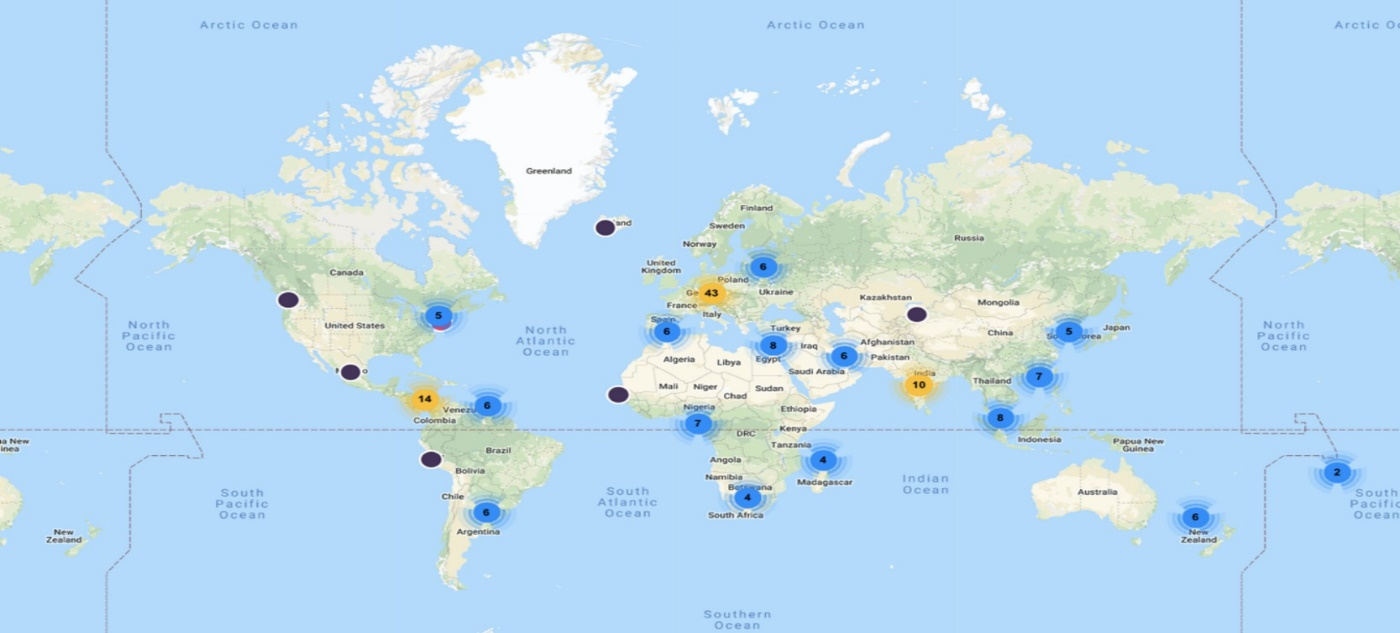
\includegraphics[width=\textwidth]{ibm_imple_around_the_world.jpg}
  \caption{IBM's implementation around the world (source: IBM)}
\end{figure}

\subsection{IBM Products and Inventions}

IBM is a multinational company that manufactures and sells computer hardware, middleware, and software, as well as providing consulting services in a variety of fields, from computer systems to nanotechnology. IBM is also a big research institution, having acquired the record for the most U.S. patents generated by a company for 28 years (as of 2020). The automated teller machine (ATM), floppy disk, hard disk drive, magnetic stripe card, relational database, SQL programming language, UPC barcode, and dynamic random-access memory (DRAM) are just a few of IBM's inventions.\footnote{\url{https://en.wikipedia.org/wiki/IBM}}

IBM's business operations have consistently moved to focus on higher-value, more profitable areas. This includes the 1991 spin-off of printer manufacturer Lexmark, the 2005 and 2014 sales of Lenovo's personal computer (ThinkPad/ThinkCentre) and x86-based server operations, and the acquisition of companies like PwC Consulting (2002), SPSS (2009), The Weather Company (2016), and Red Hat (2019). IBM announced in 2015 that it would go ``fabless,'' continuing to design semiconductors but outsourcing manufacturing to GlobalFoundries, and in 2020, the company announced the spin-off of its Global Technology Services division's Managed Infrastructure Services unit, with completion expected by the end of 2021.\footnote{\url{https://newsroom.ibm.com/mergers-and-acquisitions}}

\subsection{IBM Morocco}

IBM has had an office in Morocco for 83 years, the following timeline presents the history of IBM Morocco from its first office to its last major activities in 2017.

\begin{figure}[H]
  \centering
  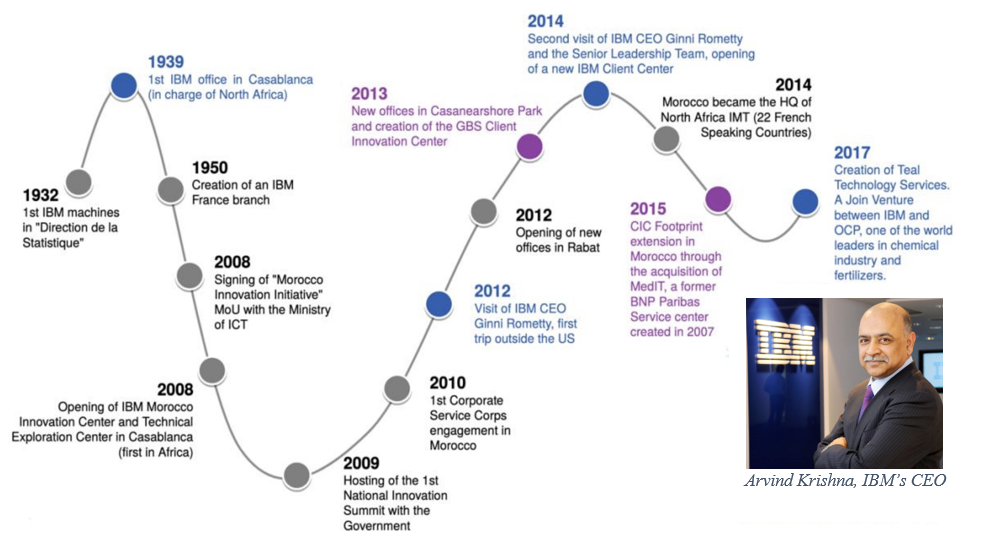
\includegraphics[width=\textwidth]{ibm_morocco_timeline.png}
  \caption{IBM Morocco timeline (source: IBM)}
\end{figure}

IBM Morocco operates in three major areas, see Figure~\ref{fig:ibm_morocco_services}:

\begin{itemize}
  \item \textbf{Global Business Services or GBS:} which means Business consulting. IBM Maroc markets and delivers specific development. It contains the CIC which is the cost center affiliated with the GBS activity. For example, if the GBS markets the projects, CIC delivers them at a lower cost.
  \item \textbf{Services for IT infrastructures or GTS (Global Technology Services)} which brings together a set of high value-added service offers to support companies in their transformation and meet their new global challenges. It is the specialized branch in hardware.

\begin{figure}[H]
  \centering
  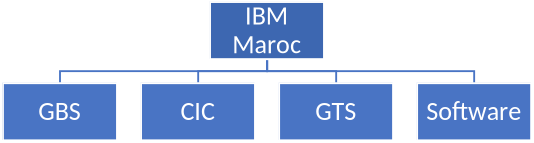
\includegraphics[width=0.5\textwidth]{ibm_morocco_services.png}
  \caption{IBM Morocco Services (source: made by me)}
  \label{fig:ibm_morocco_services}
\end{figure}
\end{itemize}

\subsection{IBM Client Innovation Center}

\subsubsection{CIC Morocco}

Since January 2015, Morocco CIC has integrated MEA Centers to leverage the right skills from different centers. The acquired company MedIT in end of 2015, was integrated to IBM in 2016 and joined GIC network in 2017. Though delivering from different locations, MEA centers share the same operations, solutioning and delivery excellence functions.

The centers based in Morocco offers clients High Value application development, application maintenance and systems integration services that address increasing demand for flexible software capability, putting focus on French speaking markets in North America, Europe, and Africa.

CIC Morocco consists of a highly motivated, experienced, and dynamic workforce planning for aggressive resource growth in 2017 supported by GBS across growth platforms.

More specifically the combined entity will ensure:
\begin{itemize}
  \item Cost optimized operations through shared support resources
  \item Synchronized capacity planning execution and fulfillment optimization --- Centralized
  \item Management reporting and communication channels
  \item Common capacity build programs synchronized with LK
\end{itemize}

\subsubsection{CIC Organizational Chart}

\begin{figure}[H]
  \centering
  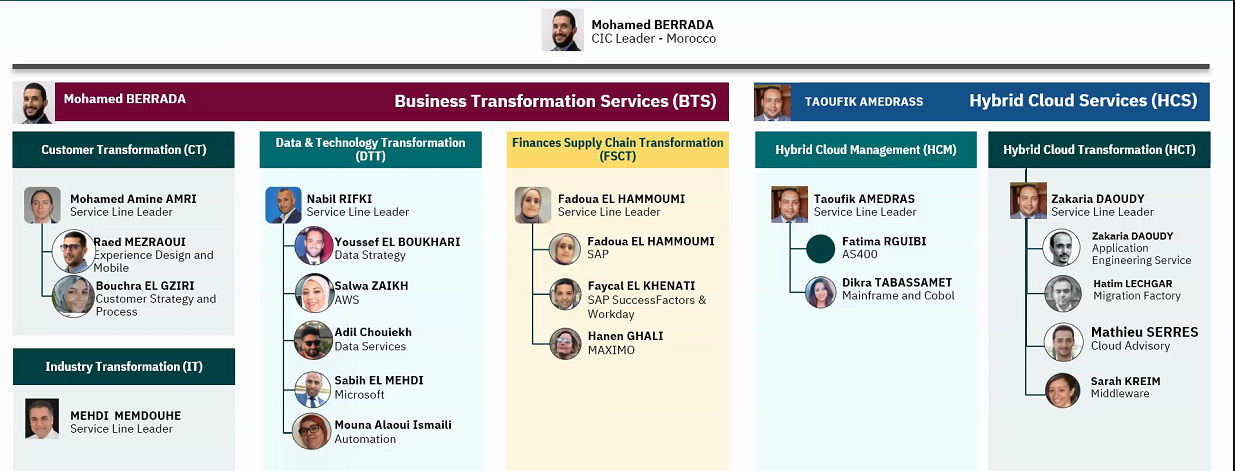
\includegraphics[width=\textwidth]{cic_org_chart.png}
  \caption{CIC Organizational Chart (source: IBM ``Confidential'')}
\end{figure}

Based on Casablanca, CIC Morocco is led by Mr. Mohamed Berrada and has two main services as follows:

\begin{itemize}
  \item Business Transformation Services (BTS)
  \item Hybrid Cloud Services (HCS)
\end{itemize}

The BTS is also led by Mr. Mohamed Berrada, and it is formed by several services for offering transformation consulting to the client such as Customer Transformation, Industry transformation, Data\&Technology Transformation (DTT), and Finances Supply chain Transformation (FSCT).

The DDT service line is led by Mr. Nabil RIFKI and composed of numerous data services including Data Strategy, Amazon Web Services (AWS), Data services, Microsoft, and Automation.

In the next section, we will present the Microsoft team and its organizational chart.

\subsection{Hakkoda: Snowflake Data Engineering Expertise}
\label{subsec:hakkoda}
\begin{figure}[H]
    \centering
    
\includegraphics[width=0.75\linewidth]{hakkoda.png}
    \caption{Hakkoda}
    \label{fig:hakkoda-logo}
\end{figure}

\textbf{Hakkoda} is a data engineering consultancy that built its reputation as one of the foremost Snowflake-specialized partners in North America and Europe. Founded with a focus on cloud data platform modernization, Hakkoda developed deep expertise in Snowflake architecture, \gls{dbt} pipeline development, data vault modeling, and DataOps automation. The company served a diverse portfolio of enterprise clients across the retail, manufacturing, financial services, and food and beverage sectors.

Hakkoda's service offering centered on helping organizations migrate from legacy on-premises data warehouses to Snowflake, design scalable data architectures, and implement \gls{cicd} practices for data engineering workflows. The firm distinguished itself from generalist consulting firms through its Snowflake-native engineering methodology and its emphasis on automation, repeatability, and governance.

In 2023, Hakkoda was acquired by IBM, a strategic move that allowed IBM to significantly reinforce its Snowflake practice capabilities within the CIC network. The acquisition brought Hakkoda's engineering talent, proprietary accelerators, and Snowflake Elite Partner status under the IBM umbrella, creating a combined offering that marries IBM's global delivery scale with Hakkoda's specialized cloud data engineering competencies.

The team responsible for the ARYZTA project operates under the Hakkoda brand within IBM, and is composed of senior Data Engineers, DataOps specialists, and Snowflake architects with extensive experience in enterprise data platform modernization. This internship was conducted within this team, contributing directly to the Snowflake environment alignment and CI/CD implementation workstream.

\subsection{ARYZTA: The Client Organization}
\label{subsec:aryzta}

\begin{figure}[H]
    \centering
    \placeholder{ARYZTA company logo}{Image to be inserted (file \texttt{aryzta.png}).}
    \caption{ARYZTA}
    \label{fig:aryzta}
\end{figure}


\textbf{ARYZTA AG} is a Swiss-Irish multinational corporation and one of the world's largest industrial bakery companies. Operating in more than 20 countries across Europe, North America, and Asia-Pacific, ARYZTA produces and distributes a wide range of frozen and fresh bakery products to quick service restaurants, food service operators, retail chains, and convenience stores. The company supplies products to some of the world's most recognized fast-food chains and employs tens of thousands of people globally.

ARYZTA's operations are characterized by high supply chain complexity, tight food safety and traceability requirements, and the need to coordinate logistics, production, and procurement across a geographically dispersed manufacturing network. This complexity generates large volumes of operational data that must be processed, integrated, and analyzed in near real-time to support decision-making across the business.

\subsubsection{Snowflake in the ARYZTA Data Ecosystem}

To address its data integration and analytics requirements, ARYZTA adopted \textbf{Snowflake} as its central cloud data platform. Snowflake's architecture---which decouples storage from compute, supports multi-cluster warehousing, and provides native data sharing capabilities---made it particularly well-suited to ARYZTA's needs for scalable, cost-efficient data processing across multiple business domains.

Within the ARYZTA data ecosystem, Snowflake serves as the integration layer for data sourced from ERP systems, logistics platforms, and commercial applications. Data pipelines load, transform, and expose curated datasets that feed downstream BI and reporting tools used by finance, operations, and supply chain teams. The Snowflake environment is therefore a mission-critical component of ARYZTA's operational infrastructure, and its stability directly affects the quality and availability of business-critical reporting.

The platform is structured around three separate Snowflake accounts---Development, User Acceptance Testing, and Production---each intended to correspond to a distinct stage in the software delivery lifecycle. As described in subsequent sections, the absence of governed deployment practices has compromised the integrity of this multi-environment architecture.

% ─────────────────────────────────────────────────────────────
\section{Project Presentation}
\label{sec:project-presentation}

\subsection{Context and Motivation}
\label{subsec:context-motivation}

The ARYZTA data platform was managed prior to Hakkoda's involvement by a third-party consultancy. During that period, the platform underwent extensive development, but without adherence to structured DevOps or DataOps practices. The absence of a version-controlled deployment workflow, combined with a culture of direct production modifications, resulted in a state of progressive environment drift that had accumulated over a period of several years.

When Hakkoda assumed responsibility for the platform, the team was confronted with a data infrastructure in which the three Snowflake environments---\texttt{DEV}, \texttt{UAT}, and \texttt{PROD}---had diverged to such a degree that \texttt{PROD} could no longer be considered a faithful replica of any formally documented state. Tables, stored procedures, tasks, streams, and views existed in production that had no counterpart in the lower environments, and vice versa. Schema structures were inconsistent across environments, and pipeline configurations had been individually tuned in production without those changes being propagated back to \texttt{DEV} or \texttt{UAT}.

This situation created a self-reinforcing problem: because \texttt{DEV} and \texttt{UAT} were not aligned with \texttt{PROD}, testing new features or changes in lower environments provided no reliable guarantee of behavior in production. As a result, engineers were routinely compelled to bypass the lower environments and apply changes directly to \texttt{PROD}---a practice that further exacerbated the drift and increased the probability of production incidents.

The business motivation for addressing these issues is straightforward: a stable, governed data platform is a prerequisite for reliable analytics, confident product development, and sustainable platform evolution. The implementation of environment synchronization and CI/CD automation is therefore not merely a technical improvement but a foundational investment in ARYZTA's data engineering capability.

\subsection{Existing Snowflake Environment Overview}
\label{subsec:existing-env}

The ARYZTA Snowflake landscape is organized around three independent accounts, each hosted on Snowflake's cloud infrastructure and corresponding to a standard software delivery environment:

\begin{table}[H]
  \centering
  \rowcolors{2}{lightgray}{white}
  \begin{tabularx}{\textwidth}{l l X}
    \toprule
    \rowcolor{ibmblue!15}
    \textbf{Environment} & \textbf{Identifier} & \textbf{Intended Purpose} \\
    \midrule
    Development    & \texttt{DEV}  & Feature development, unit testing, exploratory data modeling \\
    User Acceptance Testing & \texttt{UAT} & Integration testing, business validation, pre-production staging \\
    Production     & \texttt{PROD} & Live operational data, production pipelines, business-critical reporting \\
    \bottomrule
  \end{tabularx}
  \caption{ARYZTA Snowflake Environment Summary}
  \label{tab:env-summary}
\end{table}

Each environment contains a set of databases, schemas, tables, views, stored procedures, tasks, streams, and Snowflake stages that collectively constitute the data platform. In an ideal state, all three environments would be structurally synchronized, differing only in the data they contain and the compute resources allocated to their virtual warehouses.

Prior to the work undertaken in this internship, the actual state of the three environments deviated significantly from this ideal. The deployment workflow in use was informal and largely undocumented: changes were developed by engineers with direct access to each environment's SQL console, and deployments were executed through manual copy-paste of SQL scripts without version control, peer review, or systematic testing.

\begin{figure}
    \centering
    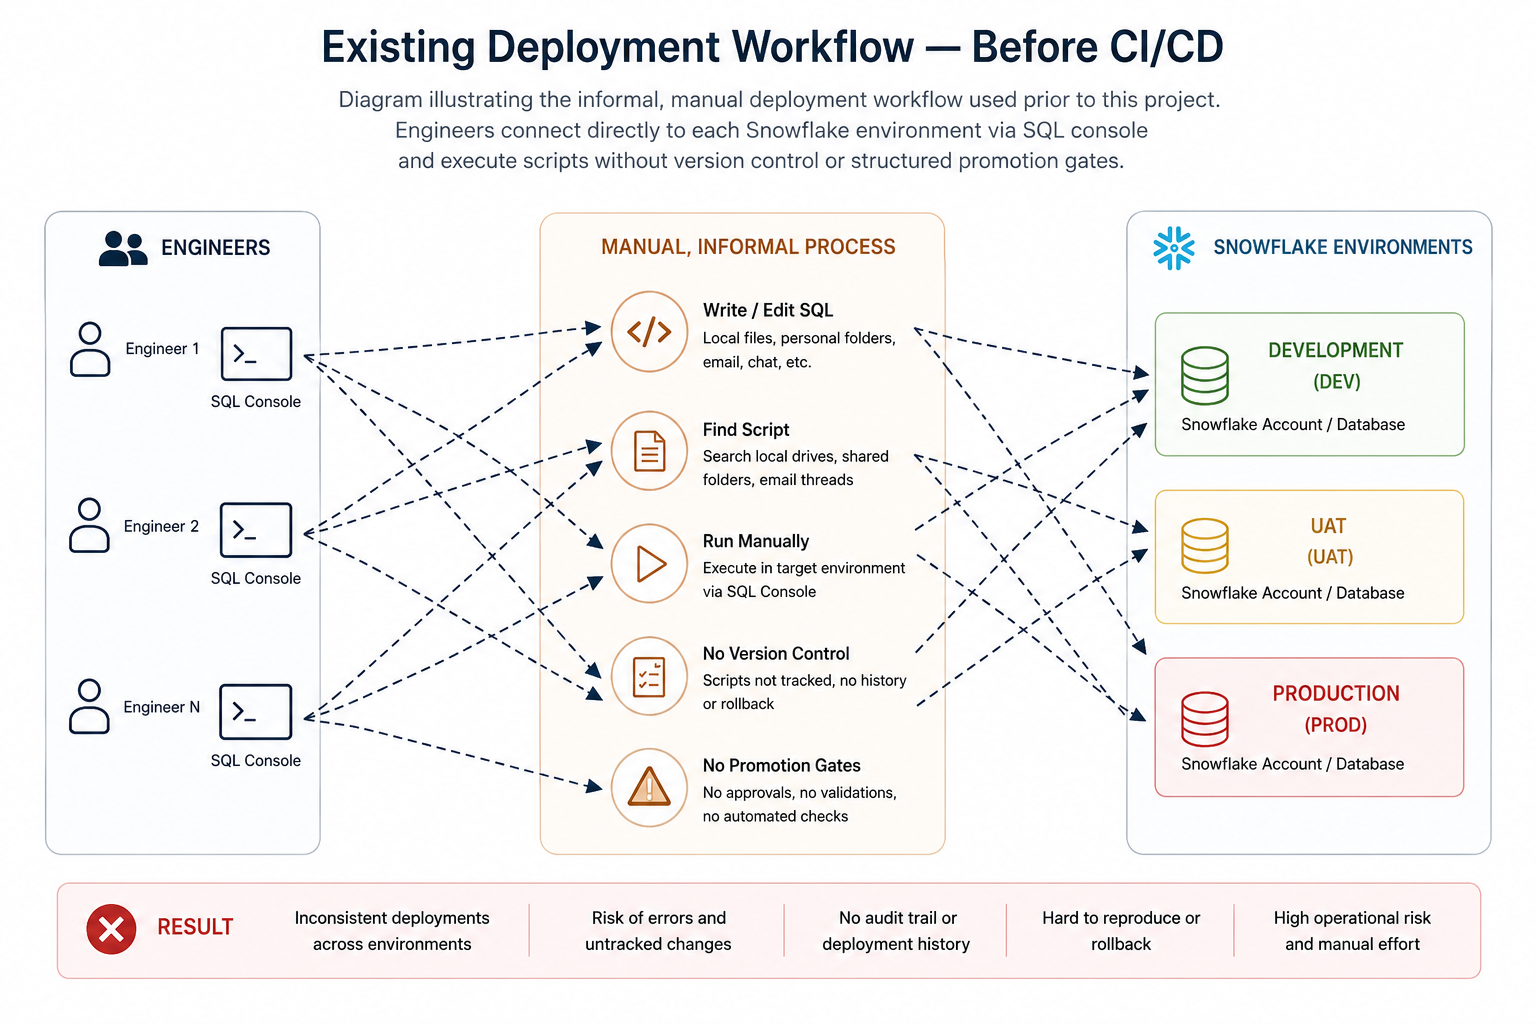
\includegraphics[width=1\linewidth]{ci_cd.png}
    \caption{Before CI/CD}
    \label{fig:placeholder}
\end{figure}

\subsection{Risks and Challenges}
\label{subsec:risks-challenges}

The combination of environment drift and ungoverned deployment practices exposes ARYZTA's data platform to a range of technical and operational risks. These may be categorized along two dimensions: deployment risk and maintenance risk.

\paragraph{Deployment Risk.} The absence of a validated lower-environment proxy for production means that the consequences of any given deployment are difficult to anticipate. A change deployed directly to \texttt{PROD} without prior testing may introduce schema conflicts, break downstream transformations, or corrupt dependent pipelines. Given the business-critical nature of the ARYZTA data platform, such incidents can directly affect operational reporting and supply chain visibility.

\paragraph{Maintenance and Auditability Risk.} Without version control, there is no definitive record of what changes were applied to each environment, by whom, and when. This makes incident debugging significantly more difficult, as engineers cannot reliably reconstruct the sequence of changes that preceded a failure. It also complicates the onboarding of new team members, who must infer the current state of the platform through direct environment inspection rather than consulting a versioned codebase.

\paragraph{Governance Risk.} The lack of \gls{rbac}-enforced deployment workflows means that any engineer with Snowflake account access can modify production objects directly. This represents a significant governance exposure, particularly in the context of data compliance requirements.

\paragraph{Scalability Risk.} As the platform evolves and the number of Snowflake objects grows, the complexity of maintaining consistency between environments through manual means increases non-linearly. Without automation, the technical debt associated with environment misalignment will continue to accumulate.

\subsection{Specific Problem Addressed}
\label{subsec:specific-problem}

Based on the preliminary assessment conducted at the outset of the internship, the specific technical problem addressed in this project can be formally defined as follows:

\begin{tcolorbox}[notebox, title={Problem Statement}]
ARYZTA's Snowflake data platform currently operates across three environments---DEV, UAT, and PROD---that have diverged significantly in schema structure, object definitions, and pipeline configuration due to years of ungoverned, manual, and undocumented deployments. The absence of a version-controlled deployment process and an automated CI/CD pipeline prevents the engineering team from safely and reproducibly promoting changes through the environment lifecycle, forcing direct production deployments and continuously increasing the risk of data platform failures.
\end{tcolorbox}

This problem encompasses the following specific technical dimensions:

\begin{enumerate}
  \item \textbf{Environment Synchronization}: DEV and UAT do not accurately reflect the PROD state, making lower-environment testing unreliable.
  \item \textbf{Missing Snowflake Objects}: Numerous tables, stored procedures, tasks, and streams exist in PROD that are absent from DEV and/or UAT.
  \item \textbf{Inconsistent Schema Definitions}: Object definitions (column types, constraints, default values) differ across environments, introducing transformation failures when deployments are attempted.
  \item \textbf{Absent Deployment Automation}: There is no automated pipeline to validate, test, and promote SQL-based changes across environments in a controlled manner.
  \item \textbf{Lack of Version Control}: No central repository tracks the authoritative state of the Snowflake codebase, making the current platform state non-reproducible.
\end{enumerate}

\subsection{Project Objectives}
\label{subsec:objectives}

In response to the identified problem, the following project objectives were formally agreed upon with the Hakkoda engineering team and the ARYZTA client stakeholders:

\begin{table}[H]
  \centering
  \rowcolors{2}{lightgray}{white}
  \begin{tabularx}{\textwidth}{c l X}
    \toprule
    \rowcolor{ibmblue!15}
    \textbf{\#} & \textbf{Objective} & \textbf{Description} \\
    \midrule
    O1 & Environment Audit       & Systematically document all discrepancies between DEV, UAT, and PROD across all Snowflake object types. \\
    O2 & Root Cause Analysis     & Identify and characterize the technical and organizational factors that led to the observed environment drift. \\
    O3 & Synchronization Strategy & Design a phased approach to bring DEV and UAT into alignment with PROD. \\
    O4 & CI/CD Pipeline          & Implement an automated deployment pipeline integrated with GitHub that enforces version-controlled promotions. \\
    O5 & GitHub Integration      & Establish a Git-based development workflow with branch protection rules and pull request review gates. \\
    O6 & Governance Framework    & Define and document deployment policies, role assignments, and environment access controls. \\
    O7 & Documentation           & Produce comprehensive technical documentation covering the architecture, the pipeline, and the onboarding process. \\
    \bottomrule
  \end{tabularx}
  \caption{Project Objectives Summary}
  \label{tab:objectives}
\end{table}

% ─────────────────────────────────────────────────────────────
\section{Project Management}
\label{sec:project-mgmt}

\subsection{Agile Methodology: SCRUM}
\label{subsec:scrum}

The project was managed in accordance with the \textbf{Agile SCRUM} framework, a widely adopted iterative methodology in software and data engineering contexts. SCRUM's emphasis on short delivery cycles, continuous feedback, and adaptive planning made it particularly well-suited to the nature of this project, where the full scope of discrepancies between environments could only be determined progressively as the investigation advanced.

The SCRUM workflow was structured around the following recurring ceremonies and artefacts:

\begin{itemize}
  \item \textbf{Sprint Planning}: At the beginning of each two-week sprint, the team reviewed the backlog and selected a set of user stories and technical tasks to be completed within the sprint. Effort estimation was conducted using story points.
  \item \textbf{Daily Stand-ups}: Short daily synchronization meetings (15 minutes) allowed team members to communicate progress, identify blockers, and coordinate cross-functional dependencies.
  \item \textbf{Sprint Reviews}: At the end of each sprint, completed deliverables were demonstrated to stakeholders, providing an opportunity for feedback and course correction.
  \item \textbf{Sprint Retrospectives}: The team reflected on the process itself---identifying what worked well, what could be improved, and what actions would be taken in the next sprint.
  \item \textbf{Backlog Refinement}: The Product Backlog was continuously groomed to ensure that upcoming stories were well-defined, estimated, and prioritized.
\end{itemize}

\subsubsection{Tooling and Collaboration Infrastructure}

The project made use of the following tools to support SCRUM execution:

\begin{table}[H]
  \centering
  \rowcolors{2}{lightgray}{white}
  \begin{tabularx}{\textwidth}{l l X}
    \toprule
    \rowcolor{ibmblue!15}
    \textbf{Tool} & \textbf{Category} & \textbf{Usage} \\
    \midrule
    ServiceNow & ITSM / Ticketing       & Sprint backlog, task tracking, incident management, change request documentation \\
    GitHub     & Version Control        & Source code repository, branch management, pull request workflow, CI/CD pipeline triggers \\
    GitHub Actions & CI/CD Automation   & Automated deployment pipeline execution, environment promotion workflows \\
    Slack      & Communication          & Team communication, sprint updates, stakeholder notifications \\
    Confluence & Documentation          & Technical documentation, architecture records, runbooks \\
    \bottomrule
  \end{tabularx}
  \caption{Project Tooling and Collaboration Infrastructure}
  \label{tab:tools}
\end{table}

The use of \textbf{ServiceNow} as the primary ticketing platform is noteworthy, as it provided traceability between individual technical tasks and the broader change management process required by ARYZTA's internal IT governance policies. Every change deployed to the PROD environment was required to be associated with a ServiceNow change request, ensuring auditability.

\subsection{Project Timeline}
\label{subsec:gantt}

The internship was structured into six sequential phases, each corresponding to a distinct set of deliverables and outcomes. The phases are described below and visualized in the Gantt chart that follows.

\begin{enumerate}
  \item \textbf{Onboarding and Environment Discovery} (Weeks 1--2): Familiarization with the Snowflake platform, IBM/Hakkoda tooling, and the ARYZTA project context. Initial access provisioning and documentation review.
  \item \textbf{Environment Audit and Discrepancy Analysis} (Weeks 3--5): Systematic comparison of DEV, UAT, and PROD environments across all object types. Documentation of all identified discrepancies in a structured audit report.
  \item \textbf{Root Cause Analysis and Strategy Design} (Weeks 6--8): Investigation of the origins of environment drift. Design of the synchronization and CI/CD strategy, including architecture decisions and tooling selection.
  \item \textbf{CI/CD Pipeline Implementation} (Weeks 9--14): Development of the automated deployment pipeline using GitHub Actions, including scripting of validation, deployment, and rollback procedures.
  \item \textbf{Environment Synchronization Execution} (Weeks 15--17): Phased application of the synchronization strategy to bring DEV and UAT into alignment with PROD.
  \item \textbf{Testing, Documentation, and Handover} (Weeks 18--20): End-to-end pipeline testing, production of technical documentation, and knowledge transfer to the ARYZTA and Hakkoda teams.
\end{enumerate}

\newpage
\begin{landscape}
\begin{figure}[H]
  \centering
  \begin{ganttchart}[
      hgrid,
      vgrid={*{6}{draw=none}, dotted},
      x unit=0.55cm,
      y unit title=0.7cm,
      y unit chart=0.65cm,
      title height=1,
      title label font=\small\bfseries,
      bar/.style={fill=ibmblue!70, rounded corners=1pt},
      bar label font=\small,
      group label font=\small\bfseries,
      milestone label font=\small,
      link/.style={->, thick, accentblue},
      bar height=0.5,
    ]{1}{20}
    \gantttitle{Internship Timeline (Weeks)}{20} \\
    \gantttitlelist{1,...,20}{1} \\

    \ganttgroup{Phase 1: Onboarding}{1}{2} \\
    \ganttbar{Environment discovery}{1}{2} \\
    \ganttbar{Tool access setup}{1}{2} \\

    \ganttgroup{Phase 2: Audit}{3}{5} \\
    \ganttbar{DEV/UAT/PROD comparison}{3}{5} \\
    \ganttbar{Discrepancy documentation}{4}{5} \\

    \ganttgroup{Phase 3: Analysis \& Design}{6}{8} \\
    \ganttbar{Root cause analysis}{6}{7} \\
    \ganttbar{Architecture design}{7}{8} \\

    \ganttgroup{Phase 4: CI/CD Implementation}{9}{14} \\
    \ganttbar{GitHub repo setup}{9}{9} \\
    \ganttbar{Pipeline scripting}{9}{13} \\
    \ganttbar{Pipeline testing}{12}{14} \\

    \ganttgroup{Phase 5: Synchronization}{15}{17} \\
    \ganttbar{DEV sync execution}{15}{16} \\
    \ganttbar{UAT sync execution}{16}{17} \\

    \ganttgroup{Phase 6: Docs \& Handover}{18}{20} \\
    \ganttbar{Technical documentation}{18}{19} \\
    \ganttbar{Knowledge transfer}{19}{20} \\
    \ganttmilestone{Final delivery}{20}

  \end{ganttchart}
  \caption{Project Gantt Chart --- Internship Timeline}
  \label{fig:gantt}
\end{figure}
\end{landscape}

\section*{Chapter Conclusion}

This chapter has established the organizational and technical foundation upon which the remainder of this report is built. The host organizations---IBM CIC Morocco and Hakkoda---bring complementary capabilities to the ARYZTA engagement: IBM's global delivery infrastructure and enterprise credibility, and Hakkoda's Snowflake-native engineering expertise. The client, ARYZTA, operates a mission-critical Snowflake data platform that has suffered from years of ungoverned deployment practices, resulting in a state of environment drift that constrains the engineering team's ability to develop and deliver platform enhancements safely.

The project objectives are clearly defined: to audit and resolve the environment discrepancies, to implement a CI/CD pipeline that enforces version-controlled deployments, and to establish a governance framework that will prevent a recurrence of the current situation. The Agile SCRUM methodology, supported by ServiceNow and GitHub, provides the structured delivery framework within which these objectives are pursued.

The following chapter presents a rigorous analysis of the current state of the platform, including a detailed characterization of the discrepancies observed, their operational impact, and the factors that gave rise to them.

\newpage


% ═══════════════════════════════════════════════════════════════
%  Chapter 2 — Problem Analysis
% ═══════════════════════════════════════════════════════════════
\chapter{Problem Analysis}
\label{chap:analysis}

\section*{Chapter Introduction}

With the project context established in the preceding chapter, this chapter undertakes a systematic and technically grounded analysis of the problem at hand. The objective is to move beyond a descriptive account of the observed discrepancies and to develop a rigorous understanding of the current state of the platform, the business consequences of its shortcomings, and the underlying factors---both organizational and technical---that produced them.

This analysis draws on the findings of the environment audit conducted during the second phase of the internship, as well as on stakeholder interviews and a review of historical deployment records. Together, these sources provide the empirical basis for the solution design presented in Chapter 3.

% ─────────────────────────────────────────────────────────────
\section{Current State Assessment}
\label{sec:current-state}

\subsection{Key Problems Identified}
\label{subsec:key-problems}

The environment audit conducted during Weeks 3--5 of the internship produced a comprehensive inventory of discrepancies between ARYZTA's three Snowflake accounts. The findings reveal a platform in which the separation between environments has, in practice, collapsed: \texttt{PROD} has become the de facto source of truth, while \texttt{DEV} and \texttt{UAT} have drifted to the point where they can no longer serve their intended functions.

The key categories of discrepancy identified are summarized in Table~\ref{tab:discrepancy-categories} and elaborated in the subsections that follow.

\begin{table}[H]
  \centering
  \rowcolors{2}{lightgray}{white}
  \begin{tabularx}{\textwidth}{l c c c X}
    \toprule
    \rowcolor{ibmblue!15}
    \textbf{Object Type}    & \textbf{DEV} & \textbf{UAT} & \textbf{PROD} & \textbf{Nature of Discrepancy} \\
    \midrule
    Tables                  & \ding{55}    & \ding{55}    & \ding{51}     & Missing columns, absent tables \\
    Stored Procedures       & \ding{55}    & \ding{55}    & \ding{51}     & Outdated logic, missing procedures \\
    Tasks                   & \ding{55}    & \ding{55}    & \ding{51}     & Missing scheduled tasks \\
    Streams                 & \ding{55}    & \ding{55}    & \ding{51}     & Change Data Capture gaps \\
    Views                   & \ding{73}    & \ding{73}    & \ding{51}     & Partial presence, definition drift \\
    Schemas                 & \ding{73}    & \ding{73}    & \ding{51}     & Structural inconsistencies \\
    Stages                  & \ding{55}    & \ding{73}    & \ding{51}     & Missing or misconfigured stages \\
    Warehouse Configuration & \ding{73}    & \ding{73}    & \ding{51}     & Size and auto-suspend differences \\
    \bottomrule
    \multicolumn{5}{l}{\footnotesize \ding{51} = Present and consistent\quad \ding{55} = Significantly absent\quad \ding{73} = Partially present or inconsistent}
  \end{tabularx}
  \caption{Summary of Snowflake Environment Discrepancies by Object Type}
  \label{tab:discrepancy-categories}
\end{table}

\subsubsection{Missing and Inconsistent Database Objects}

The most immediately impactful category of discrepancy involves database objects that exist in \texttt{PROD} but are absent from \texttt{DEV} and/or \texttt{UAT}. During the audit, a significant number of tables were found to exist exclusively in \texttt{PROD}, including several that serve as staging targets for critical data ingestion pipelines. In \texttt{DEV}, engineers attempting to develop and test enhancements to these pipelines were working against an environment that lacked the structural prerequisites for the transformation logic to execute correctly.

In addition to entirely absent objects, a substantial proportion of shared objects were found to have structurally divergent definitions. Columns had been added to \texttt{PROD} tables without the corresponding DDL being applied to the lower environments. In some cases, column data types differed between environments---an inconsistency that is particularly dangerous, as it can cause silent type-coercion failures that are difficult to detect in testing and manifest only at scale in production.

\subsubsection{Stored Procedure and Task Inconsistencies}

Snowflake stored procedures constitute a significant portion of ARYZTA's transformation logic. The audit revealed numerous instances where the procedure body in \texttt{PROD} had been modified directly---often to apply hotfixes or urgent business logic changes---without the updated version being backported to \texttt{DEV} or \texttt{UAT}. As a result, the lower environments were executing outdated procedure logic that no longer reflected the production behavior, rendering any testing conducted against these environments misleading.

Snowflake Tasks---scheduled execution units that orchestrate pipeline automation---were found to be similarly inconsistent. Several tasks defined in \texttt{PROD}, responsible for invoking stored procedures on a scheduled basis, had no counterpart in \texttt{DEV} or \texttt{UAT}. This gap meant that full end-to-end pipeline testing in a lower environment was structurally impossible.

\subsubsection{Deployment Workflow and Governance Gaps}

Beyond the object-level discrepancies, the audit identified a complete absence of formal deployment governance. There existed no documented deployment standard, no mandatory review process for Snowflake changes, and no version-controlled repository containing the authoritative DDL or DML definitions of platform objects. The deployment workflow consisted, in practice, of engineers connecting to the Snowflake web UI or SnowSQL client and executing SQL statements directly against each environment's console.

This approach had the effect of making every deployment a one-way, irreversible operation: there was no rollback mechanism, no pre-deployment validation, and no post-deployment verification step. The sole record of what had been deployed was the Snowflake query history---a per-environment log that is neither searchable across environments nor suitable for use as a source of truth for object definitions.

\begin{figure}[H]
    \centering
    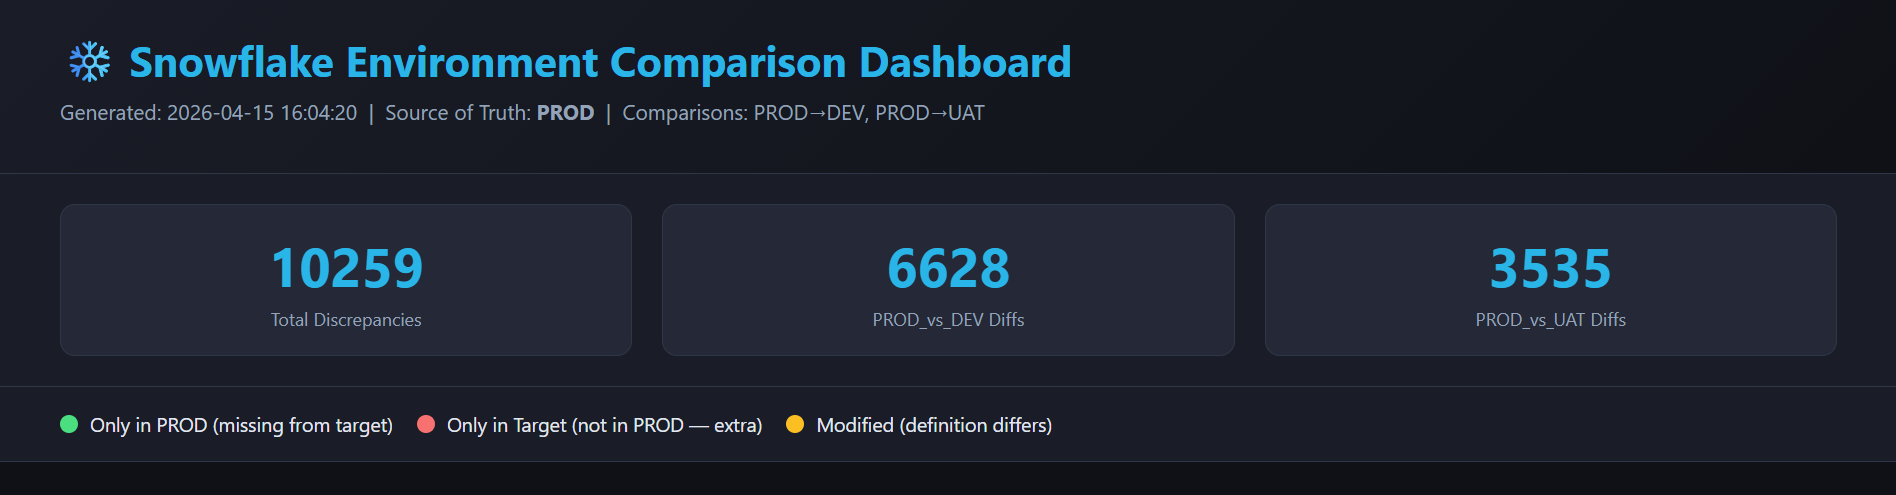
\includegraphics[width=1\linewidth]{dicrepency.png}
    \caption{Discrepancy of objects within an environment}
    \label{fig:discrepancy-objects}
\end{figure}

\begin{figure}[H]
    \centering
    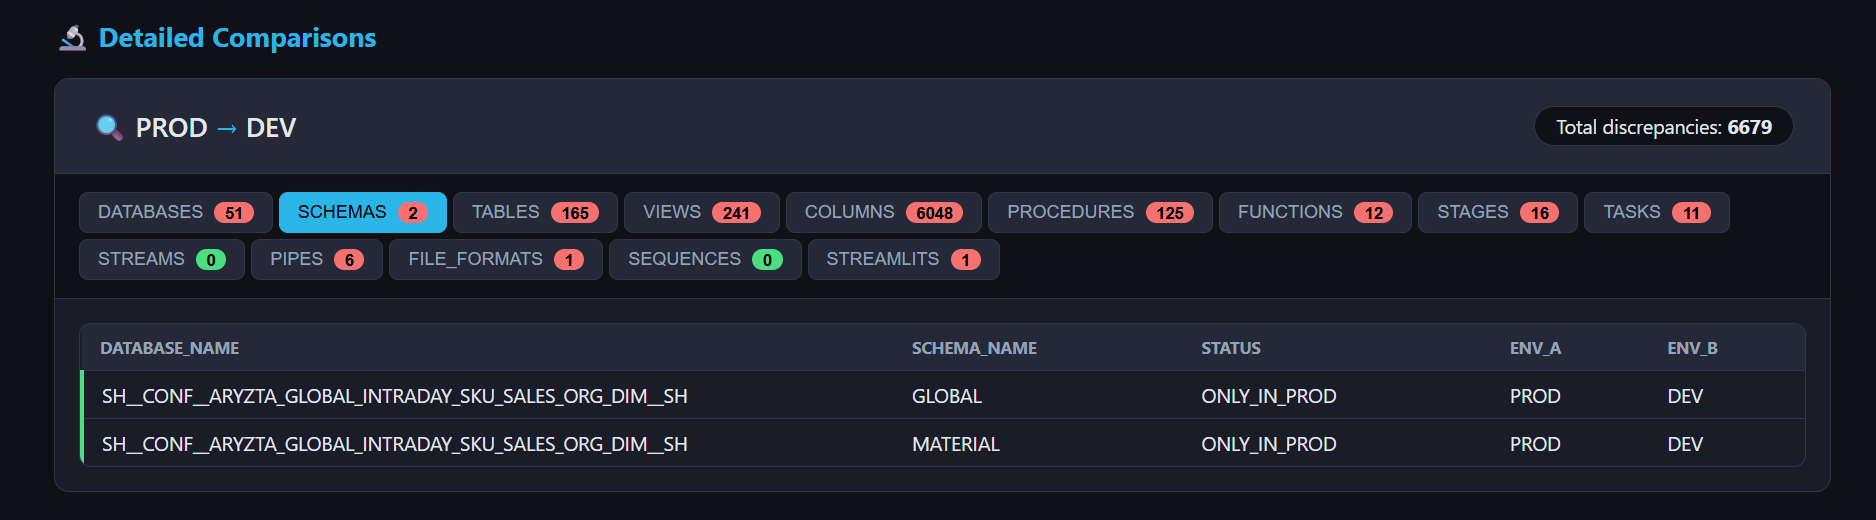
\includegraphics[width=1\linewidth]{dev_prod.png}
    \caption{Discrepancy between PROD and DEV}
    \label{fig:discrepancy-dev-prod}
\end{figure}

\begin{figure}[H]
    \centering
    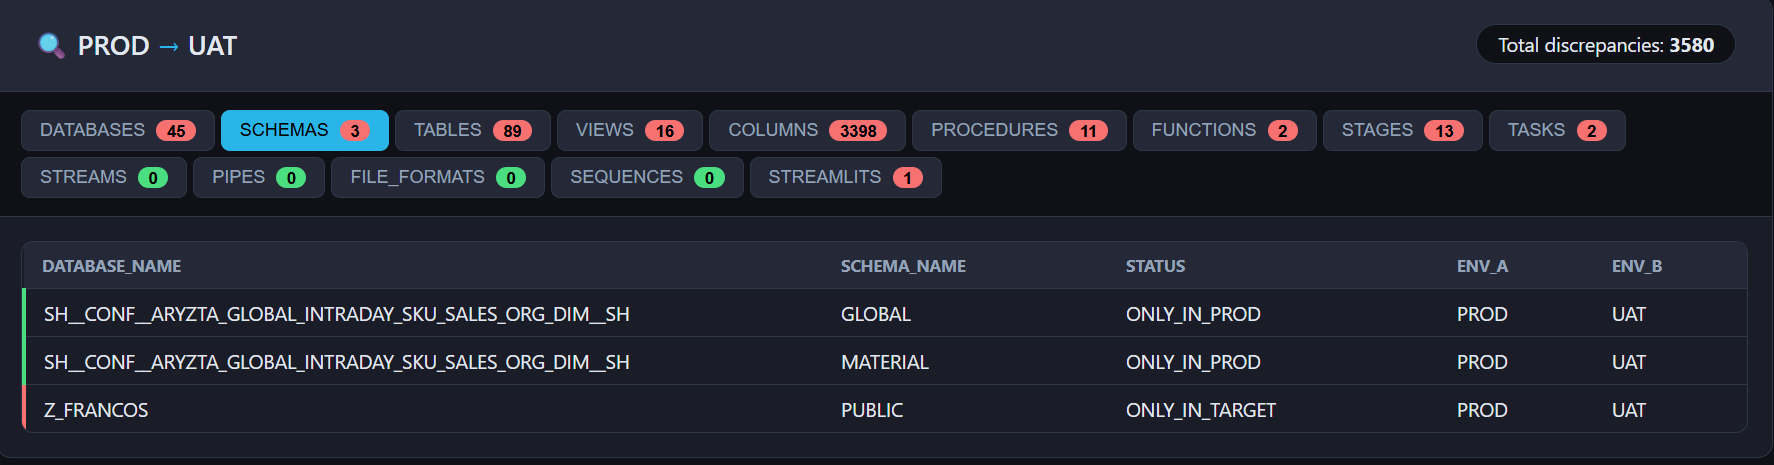
\includegraphics[width=1\linewidth]{uat_prod.png}
    \caption{Discrepancy between UAT and PROD}
    \label{fig:discrepancy-uat-prod}
\end{figure}
% ─────────────────────────────────────────────────────────────
\section{Business Impact}
\label{sec:business-impact}

\subsection{Operational Challenges}
\label{subsec:operational-challenges}

The technical state described above translates into a set of concrete operational challenges that affect the day-to-day productivity of the engineering team and the reliability of the platform for ARYZTA's business users.

\paragraph{Unreliable Development and Testing.} Because \texttt{DEV} does not accurately reflect the structure of \texttt{PROD}, features developed and tested in \texttt{DEV} carry a non-trivial probability of failure when promoted to production. Engineers are aware of this risk and have responded by shortening the development cycle---conducting only superficial testing in \texttt{DEV} before deploying directly to \texttt{PROD}---which in turn further entrenches the practice of direct production deployment.

\paragraph{Deployment Bottlenecks.} In the absence of an automated deployment pipeline, every change must be applied manually to each environment in sequence. For changes involving multiple interdependent objects---a common scenario in Snowflake platform development, where a procedure may depend on a table, which depends on a schema, which depends on a database---the risk of applying changes in the wrong order or missing a dependency is high. This complexity slows deployments and increases the cognitive load on engineers.

\paragraph{Incident Response Complexity.} When a production incident occurs---a pipeline failure, a data quality degradation, or a scheduled task error---the inability to reproduce the \texttt{PROD} state in a lower environment significantly complicates root cause analysis. Engineers cannot safely experiment with fixes in an isolated environment, as \texttt{DEV} and \texttt{UAT} do not reliably simulate \texttt{PROD} behavior.

\paragraph{Knowledge Fragmentation.} The absence of a versioned codebase means that institutional knowledge about the platform is concentrated in the individuals who have historically made changes, rather than being codified in a repository that is accessible to the full team. This creates a significant bus factor risk: if a key team member leaves or is unavailable, the team's ability to safely modify the platform is materially impaired.

\subsection{Financial and Strategic Impact}
\label{subsec:financial-impact}

While a precise financial quantification of the cost of environment misalignment is beyond the scope of this internship, the qualitative financial and strategic impacts are significant and warrant formal acknowledgment.

\paragraph{Increased Maintenance Cost.} Manual deployments are inherently more time-consuming than automated ones. The time spent by senior Data Engineers on manually executing and verifying deployments represents a direct opportunity cost: those hours could otherwise be invested in platform enhancement, data product development, or technical debt reduction.

\paragraph{Production Incident Risk.} Direct production deployments without prior validation in a synchronized lower environment dramatically increase the probability of production-impacting incidents. Data platform failures in ARYZTA's context---where operational reporting and supply chain analytics depend on the platform---can have measurable downstream consequences, including delayed decision-making and reputational risk with business stakeholders.

\paragraph{Technical Debt Accumulation.} Each ad-hoc deployment that bypasses the lower environments adds to the stock of technical debt. Resolving this debt requires progressively more engineering effort as the discrepancies between environments compound over time. The cost of not addressing environment alignment therefore increases monotonically with time.

\paragraph{Impediment to Platform Evolution.} The inability to safely test new features in a production-representative lower environment acts as a structural constraint on the pace of platform innovation. ARYZTA's data team is unable to confidently adopt new Snowflake capabilities---such as dynamic tables, Snowpark, or data sharing features---without incurring disproportionate deployment risk.

% ─────────────────────────────────────────────────────────────
\section{Root Cause Analysis}
\label{sec:root-cause}

A rigorous problem analysis requires going beyond the symptoms---the observed discrepancies---to identify the underlying causes that gave rise to them. The root cause analysis conducted in this section draws on the findings of the environment audit, stakeholder interviews with current and former members of the ARYZTA platform team, and a review of available deployment records. The analysis is organized along two complementary axes: organizational factors and technical factors.

\subsection{Organizational Factors}
\label{subsec:org-factors}

\subsubsection{Absence of a Deployment Governance Framework}

The most fundamental organizational root cause of the observed environment drift is the complete absence of a formal deployment governance framework. At no point during the previous management phase was a documented deployment standard produced, reviewed, or enforced. There was no defined process for how changes should be developed, tested, approved, and promoted across the environment lifecycle. In the absence of such a framework, individual engineers defaulted to the path of least resistance: applying changes directly to the environment in which they were needed, without regard for the downstream consequences on other environments.

Governance frameworks in data engineering contexts typically encompass deployment standards (e.g., all DDL changes must be version-controlled), access control policies (e.g., only a designated release engineer may deploy to \texttt{PROD}), and change management procedures (e.g., all \texttt{PROD} deployments require a corresponding change request ticket). None of these elements were in place for the ARYZTA platform.

\subsubsection{Weak DevOps and DataOps Culture}

The previous management team operated with a delivery model that prioritized speed of feature delivery over the engineering discipline required to sustain that delivery at scale. This orientation---common in early-stage data platform projects where time-to-value is prioritized over maintainability---is appropriate in certain contexts but becomes progressively more problematic as the platform matures and the cost of inconsistency accumulates.

The absence of a \gls{devops} culture manifested in several concrete ways: no code review process for Snowflake SQL, no environment-parity requirement in sprint acceptance criteria, no investment in deployment automation, and no retrospective analysis of deployment incidents to identify structural improvements.

\subsubsection{Insufficient Environment Management Strategy}

A three-environment architecture (\texttt{DEV}/\texttt{UAT}/\texttt{PROD}) provides value only if the environments are actively managed to remain synchronized. This requires an explicit environment management strategy that defines how changes flow between environments, how environments are refreshed, and how discrepancies are detected and remediated. The previous team had no such strategy: the three Snowflake accounts existed as independent operational entities rather than as interconnected stages of a single delivery pipeline.

\subsection{Technical Factors}
\label{subsec:tech-factors}

\subsubsection{Direct Production Deployment as Standard Practice}

The most direct technical cause of environment drift is the practice of applying changes directly to \texttt{PROD} without first deploying them to \texttt{DEV} and \texttt{UAT}. This practice was not an exceptional deviation from a defined standard---it was, in effect, the standard. As documented in the deployment history review, the majority of schema changes and stored procedure updates applied to the \texttt{PROD} environment during the previous management period have no corresponding record of prior deployment to lower environments.

The technical mechanism by which this practice perpetuates itself is straightforward: once a change is applied only to \texttt{PROD}, the lower environments become structurally incompatible with \texttt{PROD}. Any subsequent attempt to use the lower environments for testing will encounter failures or behavioral differences that engineers interpret as artifacts of the lower environment rather than as reflections of a genuine issue. This erodes confidence in the lower environments and reinforces the preference for direct \texttt{PROD} deployment.

\subsubsection{Absence of Version Control for Snowflake Objects}

No \gls{vcs} system was used to track the definitions of Snowflake objects. The DDL for tables, procedures, tasks, and other objects existed---if at all---only as informal scripts on engineers' local machines or in unstructured shared storage, without versioning, branching, or history. This absence of version control made it structurally impossible to:

\begin{itemize}
  \item Determine the authoritative current definition of any given Snowflake object.
  \item Identify what had changed between deployments.
  \item Roll back to a previous state in the event of a failed deployment.
  \item Enforce peer review of changes before deployment.
\end{itemize}

\subsubsection{No Infrastructure-as-Code Practices}

\gls{iac} practices---in which the desired state of infrastructure components is declared in version-controlled configuration files rather than applied through imperative commands---are well-established in cloud operations. In the data engineering context, this principle extends to the definition of Snowflake objects in SQL migration files or declarative configuration schemas that can be applied idempotently to any target environment. The previous team made no use of such practices: all deployments were imperative, executed through ad-hoc SQL statements with no idempotency guarantees.

\subsubsection{Lack of Deployment Automation}

The absence of any deployment automation mechanism meant that even when engineers intended to apply a change to all three environments, the process was error-prone. Manual steps were occasionally skipped, objects were deployed in incorrect dependency order, and post-deployment validations were rarely performed. Automation addresses these failure modes by encoding the correct deployment sequence and validation logic into a repeatable pipeline that executes deterministically on every invocation.



\begin{table}[H]
  \centering
  \rowcolors{2}{lightgray}{white}
  \begin{tabularx}{\textwidth}{l l X l}
    \toprule
    \rowcolor{ibmblue!15}
    \textbf{Root Cause} & \textbf{Category} & \textbf{Description} & \textbf{Impact} \\
    \midrule
    No governance framework       & Organizational & No deployment standards or policies defined             & High \\
    Weak DevOps culture           & Organizational & Speed prioritized over engineering discipline           & High \\
    No environment management     & Organizational & Environments treated as independent silos               & High \\
    Direct PROD deployments       & Technical      & Changes applied to PROD without lower-env testing       & Critical \\
    No version control            & Technical      & Object definitions not tracked in any VCS               & Critical \\
    No IaC practices              & Technical      & Imperative deployments with no idempotency guarantees   & High \\
    No deployment automation      & Technical      & Manual, error-prone deployment steps                    & High \\
    No rollback mechanism         & Technical      & No ability to revert failed deployments safely          & Medium \\
    \bottomrule
  \end{tabularx}
  \caption{Root Cause Analysis Summary}
  \label{tab:root-cause}
\end{table}

\section*{Chapter Conclusion}

This chapter has presented a comprehensive and technically rigorous analysis of the current state of ARYZTA's Snowflake data platform. The environment audit revealed systemic discrepancies across all major Snowflake object types, with \texttt{DEV} and \texttt{UAT} failing to accurately represent the \texttt{PROD} state due to years of ungoverned direct-production deployments.

The business impact of these discrepancies is substantial: unreliable testing, deployment bottlenecks, increased incident response complexity, accumulating technical debt, and an impediment to platform evolution. The root cause analysis identifies two interlocking sets of causes---organizational (absence of governance, weak DevOps culture) and technical (no version control, no IaC, no automation)---that together explain how the platform arrived at its current state.

Importantly, these root causes are not intractable. They can be systematically addressed through the implementation of a versioned codebase, an automated CI/CD pipeline, and a governance framework that enforces structured deployments. The design of this solution is the subject of the following chapter.

\newpage


% ═══════════════════════════════════════════════════════════════
%  Chapter 3 — Solution Design
% ═══════════════════════════════════════════════════════════════
%  Design chapter: architecture of the audit tool (Part A) and the
%  synchronisation strategy (Part B). Diagrams only — no source code.
%
\chapter{Solution Design}
\label{chap:design}

\section*{Chapter Introduction}

The preceding chapter established, through a systematic audit and a structured root cause analysis, that the misalignment of ARYZTA's Snowflake environments stemmed from a small number of interlocking deficiencies: the absence of version control, the lack of a deployment governance framework, and the normalisation of direct production changes. Crucially, that analysis also revealed a more immediate obstacle---the absence of any reliable instrument to \emph{measure} the extent of the drift. Before a synchronisation strategy could be designed, the team required an objective, repeatable, and above all \emph{safe} means of comparing the three environments.

This chapter presents the design of the solution in two complementary parts. \textbf{Part~A} describes the architecture of the \textbf{Snowflake Environment Comparator}, a purpose-built, strictly read-only application developed to audit and quantify the discrepancies between any two Snowflake environments. \textbf{Part~B} describes the \textbf{multi-environment synchronisation strategy}, which leverages Snowflake Secure Data Sharing and a scheduled stored procedure to restore and maintain alignment of the lower environments with \texttt{PROD}.

The two parts are deliberately sequenced to mirror the engineering logic of the project: one cannot remediate what one cannot measure. The comparator provides the diagnostic foundation---a trustworthy, auditable picture of the divergence---while the synchronisation mechanism provides the corrective action. Throughout, the design choices are justified with reference to the constraints identified in Chapters~1 and~2, in particular the over-riding requirement that no diagnostic activity may itself introduce risk to the production platform. The realisation of these designs---their concrete implementation, deployment, and the results obtained---is the subject of Chapter~4.

% ─────────────────────────────────────────────────────────────
\section{Solution Overview}
\label{sec:solution-overview}

The solution comprises two engineered artefacts that together address objectives O1 through O3 defined in Chapter~1 (environment audit, root cause analysis, and synchronisation strategy). Their roles are summarised in Table~\ref{tab:design-objectives}.

\begin{table}[H]
\centering
\small
\renewcommand{\arraystretch}{1.6}
\setlength{\tabcolsep}{8pt}
\begin{tabularx}{\textwidth}{
>{\raggedright\arraybackslash\bfseries}p{4cm}
>{\raggedright\arraybackslash}p{4.2cm}
>{\raggedright\arraybackslash}X}
\toprule
\rowcolor{ibmblue!15}
\textbf{Artefact} &
\textbf{Primary Role} &
\textbf{Objectives Addressed} \\
\midrule
Snowflake Environment Comparator &
Diagnosis and read-only comparison of Snowflake environments &
$\bullet$ \textbf{O1}: Audit of schema and data differences \newline
$\bullet$ \textbf{O2}: Identification and quantification of environment drift \\
Synchronisation Strategy &
Controlled remediation using Secure Data Sharing &
$\bullet$ \textbf{O3}: Synchronisation of \texttt{DEV} and \texttt{UAT} with \texttt{PROD} \\
\bottomrule
\end{tabularx}
\caption{Alignment between the developed artefacts and the project objectives.}
\label{tab:design-objectives}
\end{table}

The design is governed by four principles that recur throughout this chapter:

\begin{itemize}
  \item \textbf{Safety by construction.} The diagnostic tool must be incapable of altering any Snowflake environment. Read-only behaviour is enforced structurally rather than relied upon as a convention.
  \item \textbf{Reproducibility.} Both the audit and the synchronisation must yield deterministic, repeatable results so that drift can be tracked over time and remediation can be re-applied safely.
  \item \textbf{Auditability.} Every comparison run and every synchronisation action is persisted to a queryable record, providing the traceability that the previous management regime lacked.
  \item \textbf{Least intrusion on production.} \texttt{PROD} is treated as the authoritative source of truth; the synchronisation reads from it without copying or modifying its data, and the audit never writes to it at all.
\end{itemize}

% ═══════════════════════════════════════════════════════════════
\section{Audit and Comparison Tool Architecture}
\label{sec:comparator}

The \textbf{Snowflake Environment Comparator} is a single-user application that compares two Snowflake environments---designated \emph{source} and \emph{target}---and reports, for every database object in scope, one of four statuses: \texttt{MATCH}, \texttt{MISSING\_IN\_SOURCE}, \texttt{MISSING\_IN\_TARGET}, or \texttt{DRIFT}. It produces a match-rate scorecard, supports drill-down to the level of individual attributes, and retains a queryable history of past runs. The application is implemented as a Streamlit interface over a layered Python codebase, with all comparison state persisted locally in an SQLite database accessed through SQLAlchemy.

The following subsections present the architecture through three design views---the system context, the persistence data model, and the dynamics of a comparison run---followed by a description of the object types compared and the criteria applied to each.

% ── 1. System context ────────────────────────────────────────
\subsection{System Context}
\label{subsec:sys-context}

\begin{figure}[H]
  \centering
  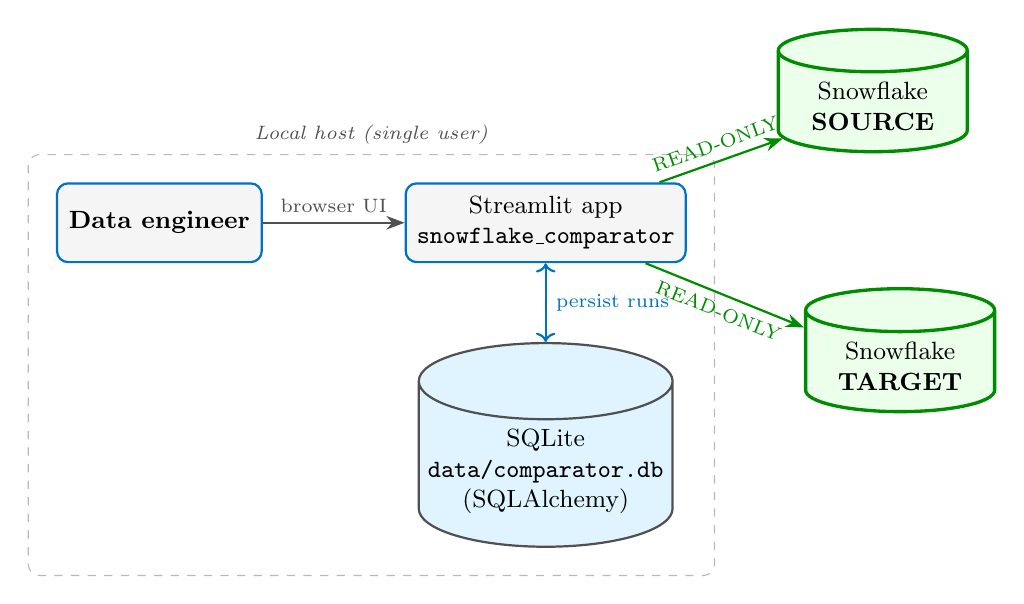
\begin{tikzpicture}[
      font=\small,
      node distance=1.0cm and 1.8cm,
      box/.style={rectangle, rounded corners, draw=accentblue, thick, fill=lightgray, align=center, minimum height=1cm, minimum width=2.6cm, inner sep=4pt},
      store/.style={cylinder, shape border rotate=90, aspect=0.3, draw=darkgray, thick, fill=snowblue!15, align=center, minimum height=1.2cm, minimum width=2.2cm},
      sf/.style={cylinder, shape border rotate=90, aspect=0.3, draw=green!55!black, very thick, fill=green!8, align=center, minimum height=1.3cm, minimum width=2.4cm},
      ro/.style={-{Stealth}, thick, green!55!black},
      rw/.style={<->, thick, accentblue},
      plain/.style={-{Stealth}, thick, darkgray},
    ]
    \node[box] (user) {\textbf{Data engineer}};
    \node[box, right=of user] (app) {Streamlit app\\\texttt{snowflake\_comparator}};
    \node[store, below=of app] (sqlite) {SQLite\\\texttt{data/comparator.db}\\(SQLAlchemy)};
    \node[sf, above right=0.4cm and 1.8cm of app] (src) {Snowflake\\\textbf{SOURCE}};
    \node[sf, below right=0.4cm and 1.8cm of app] (tgt) {Snowflake\\\textbf{TARGET}};

    \draw[plain] (user) -- node[above, font=\scriptsize] {browser UI} (app);
    \draw[rw] (app) -- node[right, font=\scriptsize] {persist runs} (sqlite);
    \draw[ro] (app) -- node[above, sloped, font=\scriptsize] {READ-ONLY} (src);
    \draw[ro] (app) -- node[below, sloped, font=\scriptsize] {READ-ONLY} (tgt);

    \begin{scope}[on background layer]
      \node[draw=darkgray!40, dashed, rounded corners, fit=(user)(app)(sqlite), inner sep=10pt, label={[font=\scriptsize\itshape, darkgray]above:Local host (single user)}] {};
    \end{scope}
  \end{tikzpicture}
  \caption{System context of the Snowflake Environment Comparator. Every connection to Snowflake is read-only (\texttt{SELECT}, \texttt{SHOW}, \texttt{DESCRIBE}); all run state is persisted locally in SQLite.}
  \label{fig:sys-context}
\end{figure}

As shown in Figure~\ref{fig:sys-context}, the comparator runs entirely on a single local host operated by one data engineer. The application connects to two independent Snowflake accounts---the \emph{source} and the \emph{target}---and persists all of its working state in a local SQLite database via SQLAlchemy. This topology was a deliberate design choice. By running locally and reading from Snowflake over the engineer's own authenticated session, the tool requires no server infrastructure, no elevated service account, and no standing footprint inside the ARYZTA environments. The most important property of this context, however, is annotated on the arrows themselves: every interaction with Snowflake is \emph{read-only}. The application issues only \texttt{SELECT}, \texttt{SHOW}, and \texttt{DESCRIBE} statements; it never emits \gls{ddl}, \gls{dml}, \texttt{CALL}, \texttt{USE}, or \texttt{ALTER}. This guarantee is enforced structurally---by a client-side allow-list that rejects any non-read statement before it can be transmitted---which is what makes the tool safe to point directly at the production account.

% ── 2. Data model (ER) ───────────────────────────────────────
\subsection{Persistence Data Model}
\label{subsec:datamodel}

\begin{figure}[H]
    \centering
    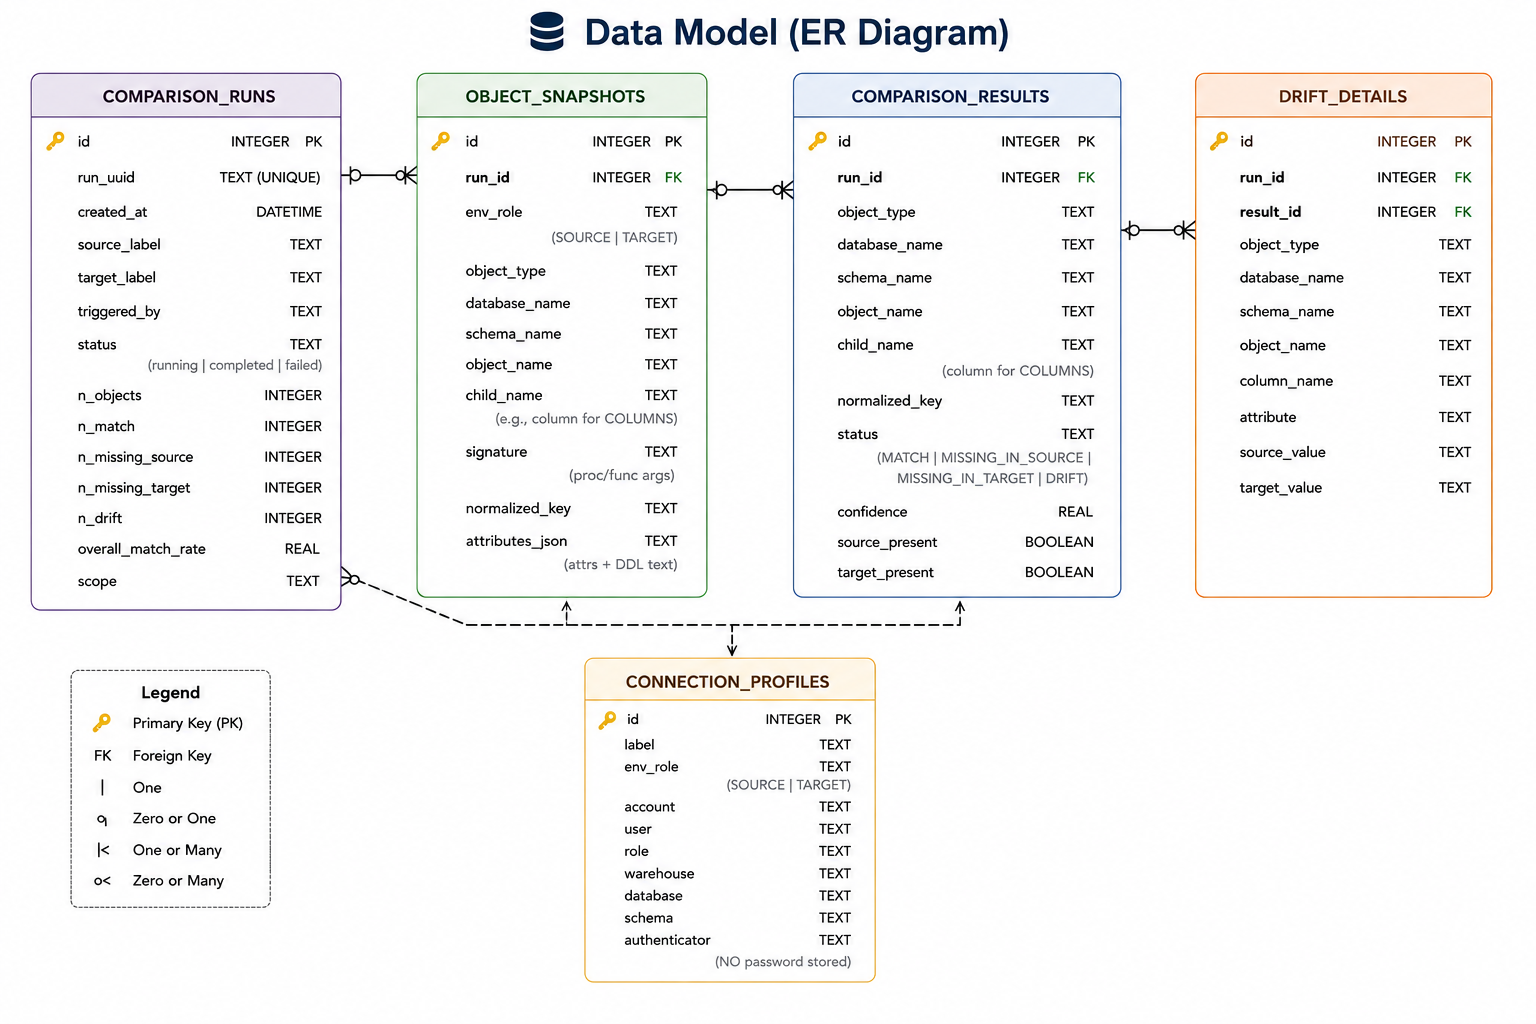
\includegraphics[width=\linewidth]{Data_Model.png}
    \caption{Entity--relationship model of the comparator's SQLite store. A \texttt{comparison\_runs} record is the parent of the object snapshots, comparison results, and drift details captured during a run.}
    \label{fig:ermodel}
\end{figure}

The comparator persists every run rather than writing transient flat files, so that history survives application restarts and can be queried after the fact. The relational model, shown in Figure~\ref{fig:ermodel}, is centred on the \texttt{comparison\_runs} entity, which records the metadata and aggregate scorecard of a single comparison and acts as the parent of three child entities. Table~\ref{tab:data-dictionary} summarises the role of each entity.

\begin{table}[H]
  \centering
  \rowcolors{2}{lightgray}{white}
  \begin{tabularx}{\textwidth}{l X}
    \toprule
    \rowcolor{ibmblue!15}
    \textbf{Entity} & \textbf{Purpose and Key Contents} \\
    \midrule
    \texttt{comparison\_runs}    & One row per comparison run: UUID, timestamp, source/target labels, status (\texttt{running}/\texttt{completed}/\texttt{failed}), object counts, per-status tallies, and the overall match rate. \\
    \texttt{object\_snapshots}   & The captured state of every object on each side (\texttt{SOURCE}/\texttt{TARGET}): type, fully qualified name, optional child name (e.g.\ a column), procedure/function signature, normalised key, and an attributes/DDL payload. \\
    \texttt{comparison\_results} & The per-object verdict: normalised key, computed status (\texttt{MATCH}, \texttt{MISSING\_IN\_SOURCE}, \texttt{MISSING\_IN\_TARGET}, \texttt{DRIFT}), a confidence score, and presence flags for each side. \\
    \texttt{drift\_details}      & For each drifted object, one row per differing attribute or column: the attribute name and its source and target values. \\
    \texttt{connection\_profiles}& Non-secret connection prefill only (account, user, role, warehouse, database, schema, authenticator). \textbf{No password is ever stored.} \\
    \bottomrule
  \end{tabularx}
  \caption{Data dictionary of the comparator's persistence model.}
  \label{tab:data-dictionary}
\end{table}

This schema embodies the auditability principle: because results and their supporting drift details are normalised and persisted, the platform team can answer questions such as ``which objects diverged between \texttt{UAT} and \texttt{PROD} on a given date, and exactly which attributes differed?'' long after the run completes. The deliberate exclusion of passwords from \texttt{connection\_profiles}---only non-secret prefill values are retained---reflects the security posture of the tool; credentials live only in the in-memory session and are never written to disk.

% ── 3. Comparison run (sequence) ─────────────────────────────
\subsection{Comparison Run Dynamics}
\label{subsec:seq-run}

\begin{figure}[H]
    \centering
    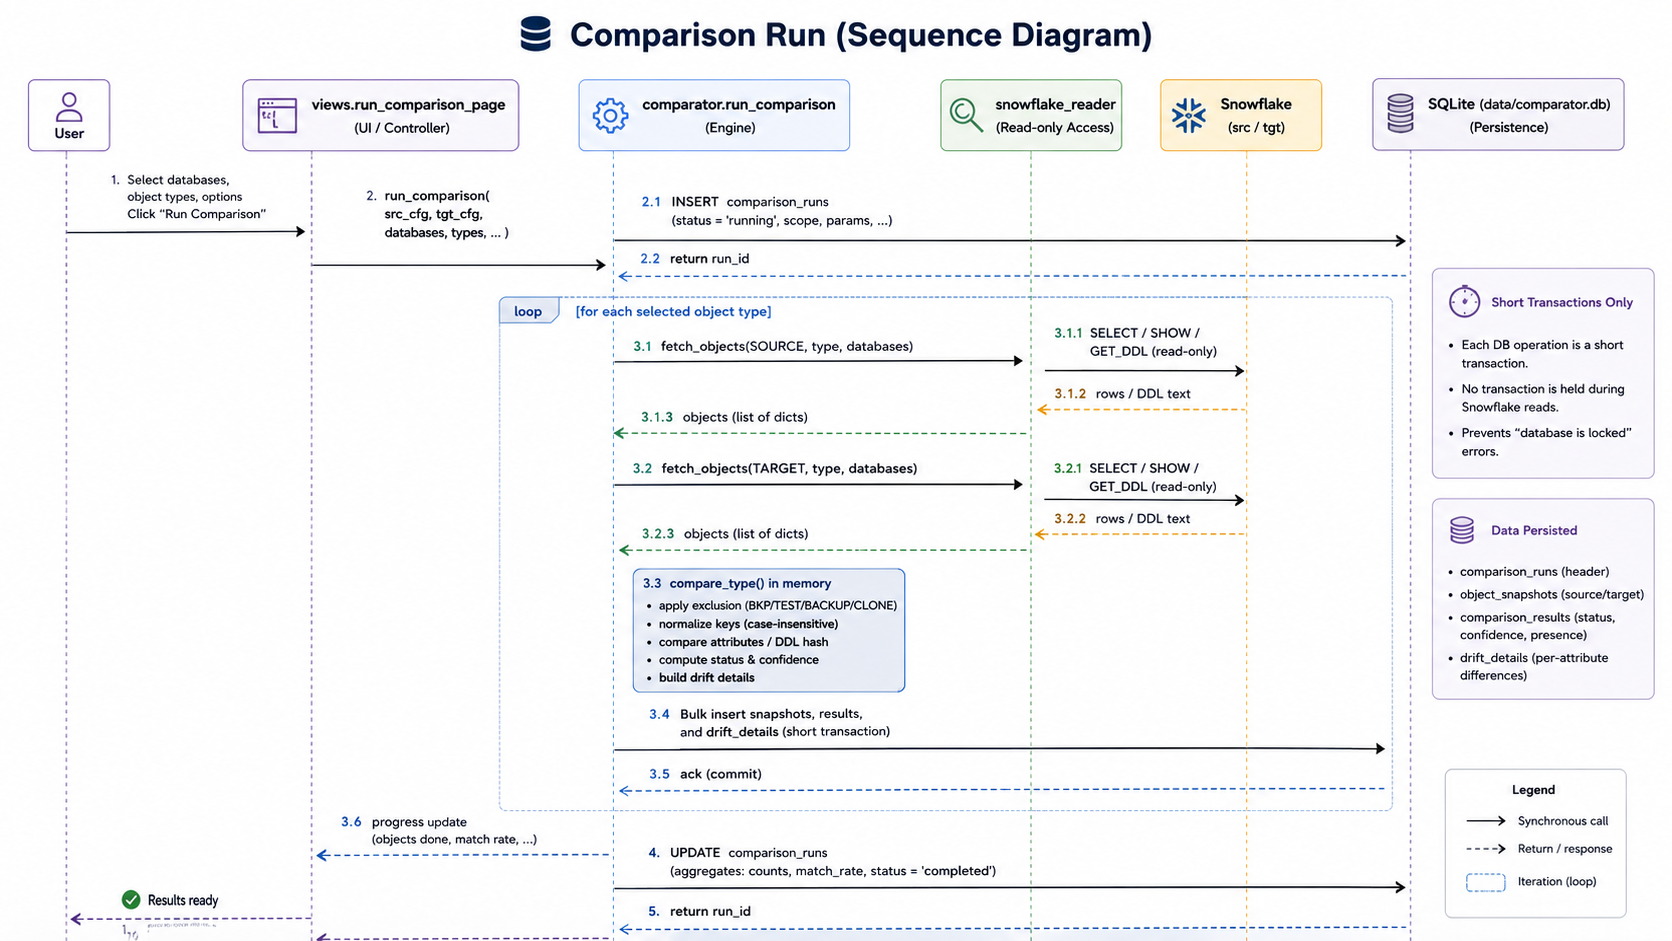
\includegraphics[width=\linewidth]{run_sequence.png}
    \caption{Sequence of a comparison run. For each object type the engine fetches the source and target objects through the read-only reader, compares them in memory, and persists snapshots, results, and drift in short transactions. No SQLite lock is held during the Snowflake reads.}
    \label{fig:seq-run}
\end{figure}

Figure~\ref{fig:seq-run} traces the dynamic behaviour of a comparison run. When the engineer selects the databases and object types and launches a run, the engine first records a run with status \texttt{running}. It then iterates over the requested object types: for each type it fetches the objects from the source and from the target through the read-only reader, compares them in memory, and writes the resulting snapshots, results, and drift details. A deliberate design refinement is that \emph{no SQLite lock is held while a Snowflake read is in flight}: transactions are kept short and are opened only around the writes. This separation avoids a database-contention condition that arises when a long network read is wrapped inside an open local transaction, and it keeps the interface responsive during runs over large schemas. On completion, the run is updated with the aggregate counts and a status of \texttt{completed}.

% ── Object types and criteria ────────────────────────────────
\subsection{Object Types and Comparison Criteria}
\label{subsec:object-criteria}

The comparator covers the full range of object types that constitute the ARYZTA platform. The criterion by which each is compared is chosen to suit its nature, as summarised in Table~\ref{tab:object-criteria}. Code-bearing objects are compared by a \emph{normalised DDL hash}, which neutralises insignificant formatting differences (whitespace, casing, comments) so that only semantically meaningful divergence is reported as drift. Structural objects are compared by their defining attributes, and columns---the finest level of granularity---are compared across seven properties.

\begin{table}[H]
\centering
\small
\renewcommand{\arraystretch}{1.45}
\setlength{\tabcolsep}{10pt}
\rowcolors{2}{lightgray}{white}
\begin{tabularx}{\textwidth}{
>{\raggedright\arraybackslash\bfseries}p{4.7cm}
X}
\toprule
\rowcolor{ibmblue!15}
\textbf{Object Category} &
\textbf{Comparison Criterion} \\
\midrule
Code Objects (\texttt{VIEWS}, \texttt{PROCEDURES}, \texttt{FUNCTIONS}, \texttt{TASKS}, \texttt{PIPES})
&
Comparison is based on a normalised DDL hash that is insensitive to formatting differences. For procedures and functions, the argument signature is also incorporated into the comparison. \\
Structural Objects (\texttt{TABLES}, \texttt{STAGES}, \texttt{STREAMS}, \texttt{SEQUENCES})
&
Comparison relies on the defining metadata attributes of each object. \\
Column Metadata (\texttt{COLUMNS})
&
Comparison includes the data type, length, precision, scale, nullability, default value, and ordinal position of each column. \\
\bottomrule
\end{tabularx}
\caption{Comparison criteria used for each supported Snowflake object category.}
\label{tab:object-criteria}
\end{table}

The complete set of object types covered is: \texttt{TABLES}, \texttt{COLUMNS}, \texttt{VIEWS}, \texttt{PROCEDURES}, \texttt{FUNCTIONS}, \texttt{STAGES}, \texttt{TASKS}, \texttt{STREAMS}, \texttt{SEQUENCES}, and \texttt{PIPES}. This breadth is what allows the audit to substantiate, with object-level evidence, the categories of discrepancy reported qualitatively in Chapter~2.

% ═══════════════════════════════════════════════════════════════
\section{Multi-Environment Synchronisation Strategy}
\label{sec:sync}

Where the comparator \emph{diagnoses} drift, the synchronisation strategy \emph{remediates} it. This section presents the design of the mechanism that realigns \texttt{DEV} and \texttt{UAT} with \texttt{PROD} and keeps them aligned on an ongoing basis.

\subsection{Design Rationale and Scope}
\label{subsec:sync-rationale}

Because no robust documentation of the platform existed---itself a consequence of the governance gaps analysed in Chapter~2---the scope of the synchronisation could not be derived from a design specification. Instead, it was defined empirically: the strategy targets \emph{every database touched by the main DAG of Snowflake tasks}, the backbone schedule that performs all processing and populates the platform's outputs. This yielded a well-bounded set of \textbf{14 databases and their schemas}, enumerated in Table~\ref{tab:sync-databases}. Scoping to the main DAG ensures that the synchronisation covers exactly the objects on which the platform's behaviour actually depends, without attempting to reconcile incidental or abandoned objects whose alignment carries no operational value.

The chosen mechanism is \textbf{Snowflake Secure Data Sharing}. A share is created \emph{from} \texttt{PROD}, which acts as the provider, and is consumed \emph{by} \texttt{UAT} and \emph{by} \texttt{DEV}, which act as consumers (\texttt{PROD} $\rightarrow$ \texttt{UAT} and \texttt{PROD} $\rightarrow$ \texttt{DEV}). Secure Data Sharing was selected for several reasons that align directly with the design principles of Section~\ref{sec:solution-overview}:

\begin{itemize}
  \item \textbf{Zero-copy, no egress.} A share exposes live, read-only references to the provider's data without physically copying it, so synchronising from \texttt{PROD} incurs no data movement, no storage duplication of the source, and no egress cost on the provider side.
  \item \textbf{Production remains authoritative and untouched.} The consumers read from the share; the provider's objects are never modified by the synchronisation, preserving \texttt{PROD} as the single source of truth.
  \item \textbf{Always current.} Because the share references live \texttt{PROD} data, each synchronisation run reflects the current production state rather than a stale snapshot.
\end{itemize}

Each of the 14 databases is exposed through its own dedicated share, following the naming convention \texttt{SH\_<DATABASE>}. On the consumer side, each share is mounted as a local database against which the synchronisation procedure reads.

\begin{table}[H]
  \centering
  \scriptsize
  \rowcolors{2}{lightgray}{white}
  \begin{tabularx}{\textwidth}{@{}c >{\ttfamily}p{4.9cm} >{\ttfamily}p{2.7cm} X@{}}
    \toprule
    \rowcolor{ibmblue!15}
    \normalfont\textbf{\#} & \normalfont\textbf{Database} & \normalfont\textbf{Schema} & \normalfont\textbf{Origin (main-DAG procedure)} \\
    \midrule
    1  & TRN\_\_CONTROLLING\_PROFITABILITY & PROFITABILITY & All procedures (home schema) \\
    2  & LOG\_\_CONTROLLING\_PROFITABILITY & LOG & Logging framework (all procedures) \\
    3  & CUR\_\_SAPECC & SAP\_ECC & \texttt{LEGAL\_ENTITY\_PRC} \\
    4  & TRN\_\_DEP\_MIGRATION & MIGRATION & \texttt{LEGAL\_ENTITY\_PRC} \\
    5  & CUR\_\_EXCELERATOR & EXCELERATOR & \texttt{COGS\_NON\_SAP\_PRC} \\
    6  & CUR\_\_EXCEL & FILES & \texttt{ACTIVITY\_ANALYSIS\_PRC} \\
    7  & RAW\_\_EXCEL & FILES & \texttt{COMPANY\_MASTER\_EXCEL\_RELOAD\_PRC} \\
    8  & CONF\_\_ARYZTA\_GLOBAL\_INTRADAY & GLOBAL & \texttt{CUST\_BUDGET\_FORECAST\_PRC} \\
    9  & CONF\_\_ARYZTA\_GLOBAL\_INTRADAY & MATERIAL & \texttt{CUSTOMER\_PROFITABILITY\_PRC} \\
    10 & CONF\_\_CONTROLLING\_PROFITABILITY & GENERAL & \texttt{CUSTOMER\_PROFITABILITY\_PRC} \\
    11 & RAW\_\_EXCELERATOR & EXCELERATOR & \texttt{MATERIAL\_COST\_LOAD\_PRC} \\
    12 & SH\_\_OUTBOUND\_\_GROSS\_TO\_NET\_INTRADAY\_\_SH & GROSS\_TO\_NET\_FACTS & \texttt{REV\_QTY\_SOLD\_SAP\_PRC} \\
    13 & SH\_\_CUR\_\_AFAS\_SNOWFLAKE\_\_SH & AFAS & \texttt{REV\_QTY\_SOLD\_ALL\_PRC} \\
    14 & CONF\_\_ORGANIZATION\_INTRADAY & ORGANIZATION & \texttt{REV\_QTY\_SOLD\_SAP\_PRC} \\
    \bottomrule
  \end{tabularx}
  \caption{Databases and schemas in synchronisation scope (derived from the main task DAG). Each database is exposed through its own share, following the naming convention \texttt{SH\_<DATABASE>}.}
  \label{tab:sync-databases}
\end{table}

\subsection{Share-Based Synchronisation Architecture}
\label{subsec:sync-arch}

\begin{figure}[H]
  \centering
  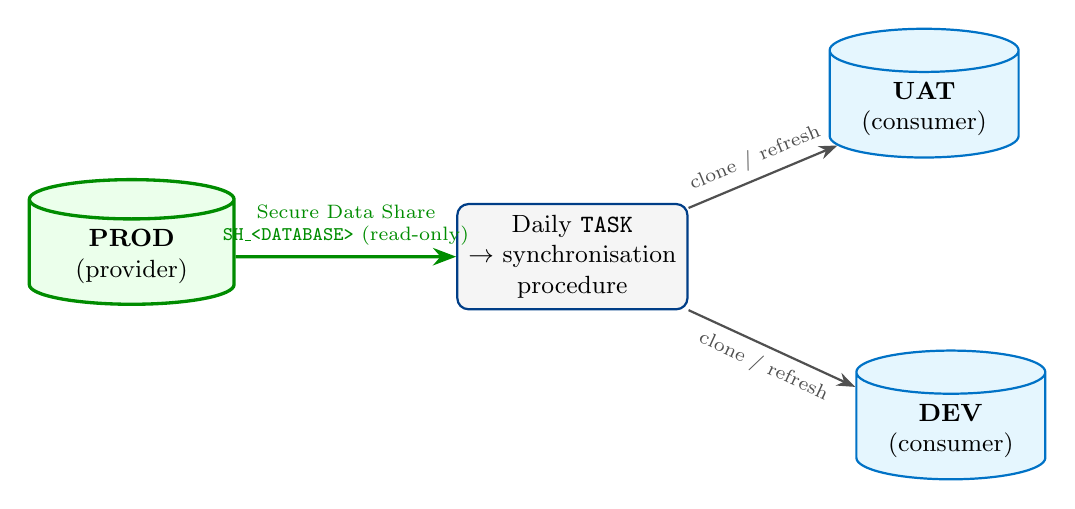
\begin{tikzpicture}[
      font=\small,
      node distance=1.4cm and 2.4cm,
      prod/.style={cylinder, shape border rotate=90, aspect=0.3, draw=green!55!black, very thick, fill=green!8, align=center, minimum height=1.4cm, minimum width=2.6cm},
      env/.style={cylinder, shape border rotate=90, aspect=0.3, draw=accentblue, thick, fill=snowblue!12, align=center, minimum height=1.3cm, minimum width=2.4cm},
      proc/.style={rectangle, rounded corners, draw=ibmblue, thick, fill=lightgray, align=center, minimum height=0.9cm, inner sep=4pt},
      edge/.style={-{Stealth}, thick, darkgray},
      share/.style={-{Stealth}, very thick, green!55!black},
    ]
    \node[prod] (prod) {\textbf{PROD}\\(provider)};
    \node[proc, right=2.8cm of prod] (task) {Daily \texttt{TASK}\\$\rightarrow$ synchronisation\\procedure};
    \node[env, above right=0.6cm and 2.4cm of task] (uat) {\textbf{UAT}\\(consumer)};
    \node[env, below right=0.6cm and 2.4cm of task] (dev) {\textbf{DEV}\\(consumer)};

    \draw[share] (prod) -- node[above, font=\scriptsize, align=center] {Secure Data Share\\\texttt{SH\_<DATABASE>} (read-only)} (task);
    \draw[edge] (task) -- node[above, sloped, font=\scriptsize] {clone / refresh} (uat);
    \draw[edge] (task) -- node[below, sloped, font=\scriptsize] {clone / refresh} (dev);
  \end{tikzpicture}
  \caption{Share-based synchronisation architecture. \texttt{PROD} provides a per-database read-only share; a daily task invokes the synchronisation procedure, which refreshes the corresponding schemas in the \texttt{UAT} and \texttt{DEV} consumer accounts.}
  \label{fig:share-flow}
\end{figure}

Figure~\ref{fig:share-flow} depicts the runtime architecture. \texttt{PROD} publishes one read-only share per in-scope database. In each consumer account, a Snowflake \texttt{TASK} runs daily and invokes a synchronisation procedure, which reads from the mounted share and refreshes the target schema. The procedure is invoked once per (source-schema, target-schema) pair: it is given the share-mounted source schema, the local target schema, and an optional list of tables to exclude from the refresh (such as operational control tables that must be preserved).

\subsection{Synchronisation Mechanism}
\label{subsec:sync-mechanism}

The synchronisation procedure accepts a source schema, a target schema, and an optional exclusion list. It operates in two phases and records every action it takes in a returnable log table, so that each run is self-documenting.

\paragraph{Phase 1 --- Clone missing tables.} The procedure enumerates the base tables present in the source schema but absent from the target (honouring the exclusion list) and recreates each one in the target by cloning it from the source. Where a direct clone is not possible---most notably for tables that are themselves read from a share---it falls back to a create-table-as-select operation. Each outcome is recorded in the log as \emph{cloned}, \emph{created via CTAS}, or \emph{error}.

\paragraph{Phase 2 --- Reconcile common tables.} For tables present in both schemas, the procedure compares their column sets (name and data type) against the source. If the structures are \emph{identical}, the target table is refreshed from \texttt{PROD} (a clone-replace, again with a create-table-as-select fallback for shared tables), bringing its data into line with production. If the structures \emph{differ}, the procedure deliberately does \emph{not} overwrite the target; instead it logs each discrepancy---\emph{only in source}, \emph{only in target}, or \emph{data-type mismatch}---under a \emph{structure mismatch} action.

This log-only treatment of structural mismatches is a central safety property of the design: the daily synchronisation refreshes data wherever it is structurally safe to do so, but it never silently reshapes a divergent table. Structural divergence is surfaced for human review---and resolved through the governed deployment pipeline described in Chapter~4---rather than being resolved automatically, which prevents the synchronisation from masking the very drift it is meant to expose.

\subsection{Idempotency and Safety Properties}
\label{subsec:sync-safety}

The synchronisation design exhibits four properties that directly counter the deficiencies identified in Chapter~2:

\begin{itemize}
  \item \textbf{Idempotent refresh.} Re-cloning a structurally identical table yields the same result regardless of how many times the daily task runs, so repeated execution is safe and convergent.
  \item \textbf{Non-destructive on divergence.} Structurally mismatched tables are logged, never overwritten, ensuring the synchronisation cannot itself destroy or silently reshape data.
  \item \textbf{Configurable exclusions.} Operational tables that must not be overwritten---such as user-maintained control tables---are passed as an exclusion list and skipped entirely.
  \item \textbf{Self-documenting runs.} Every action is recorded in the returned log table, providing the per-run auditability that the platform previously lacked.
\end{itemize}

Taken together, the comparator and the synchronisation procedure form a closed diagnostic--corrective loop: the comparator measures the drift between any two environments, and the synchronisation reduces it on a daily basis while reporting any divergence it cannot safely resolve back to the engineering team.

% ═══════════════════════════════════════════════════════════════
\section*{Chapter Conclusion}

This chapter has presented the design of the two artefacts at the heart of the solution. The Snowflake Environment Comparator was designed as a strictly read-only, layered application that ingests object metadata from any two Snowflake environments, classifies every object as \texttt{MATCH}, \texttt{DRIFT}, or one of two \texttt{MISSING} states, and persists a fully auditable history of each comparison. Its defining property---structural enforcement of read-only access---makes it safe to operate directly against the production account, satisfying the project's over-riding constraint that diagnosis must never endanger the platform. The synchronisation strategy was designed around Snowflake Secure Data Sharing, with \texttt{PROD} as an untouched provider and \texttt{DEV} and \texttt{UAT} as consumers, driven by a daily task that invokes a two-phase procedure to refresh aligned tables idempotently while surfacing structural divergence for review rather than overwriting it.

Together, these designs translate the root causes identified in Chapter~2 into concrete, engineered countermeasures: reproducible measurement in place of guesswork, and governed, non-destructive realignment in place of ad-hoc direct-to-production changes. The following chapter, \textbf{Chapter~4 --- Implementation}, details the realisation of these designs and presents the delivered solution through its operational interfaces.

\newpage


% ═══════════════════════════════════════════════════════════════
%  Chapter 4 — Implementation
% ═══════════════════════════════════════════════════════════════
%  Realisation chapter: presented through the delivered artefacts and
%  their operational interfaces (screenshots). No source code is shown,
%  in keeping with the conventions of an academic engineering report.
%
\chapter{Implementation}
\label{chap:implementation}

\section*{Chapter Introduction}

Chapter~3 established the design of the two engineered artefacts---the read-only audit tool and the share-based synchronisation mechanism---together with the governance model required to sustain them. This chapter documents their concrete realisation. Rather than reproducing source code, it presents the delivered solution as an engineer and a stakeholder actually experience it: through its operational interfaces and the evidence of its execution. The implementation is organised into three workstreams, each corresponding to one of the project's principal deliverables:

\begin{enumerate}
  \item the \textbf{Snowflake Environment Comparator}, the read-only diagnostic application, presented through its operating screens;
  \item the \textbf{version control and \gls{cicd} pipeline} integrating GitHub and GitHub Actions with the Snowflake environments; and
  \item the \textbf{synchronisation solution}---the Secure Data Shares and the scheduled procedure that drives the realignment of the lower environments.
\end{enumerate}

Throughout, attention is paid to the two constraints that have governed the project: the diagnostic tooling must remain incapable of modifying any environment, and all deployments to the environments must flow through a governed, version-controlled process rather than the ad-hoc direct changes that produced the original drift.

% ─────────────────────────────────────────────────────────────
\section{Implementation Environment and Tooling}
\label{sec:impl-env}

The implementation was carried out using the technology stack summarised in Table~\ref{tab:impl-stack}. The choices reflect the design commitments made in Chapter~3: a lightweight, locally hosted application for the audit tool, a Git-based collaboration model for source control, and GitHub Actions as the automation substrate for deployments to Snowflake.

\begin{table}[H]
  \centering
  \rowcolors{2}{lightgray}{white}
  \begin{tabularx}{\textwidth}{l l X}
    \toprule
    \rowcolor{ibmblue!15}
    \textbf{Component} & \textbf{Technology} & \textbf{Role in the Implementation} \\
    \midrule
    Application runtime & Python, Streamlit & The comparator's interface and logic (connection gate, run, results, history). \\
    Persistence & SQLite + SQLAlchemy & Local storage of comparison runs, snapshots, results, and drift. \\
    Snowflake access & Snowflake Python connector & Read-only metadata access for the comparator; authenticated deployment for the pipeline. \\
    Version control & Git + GitHub & Authoritative repository for Snowflake code, with branch protection and pull-request review. \\
    Automation & GitHub Actions & \gls{cicd} workflow: validation, environment-scoped deployment, and post-deployment checks. \\
    Change management & ServiceNow & Change-request tracking for every promotion to \texttt{PROD}. \\
    Data platform & Snowflake & The three target environments (\texttt{DEV}, \texttt{UAT}, \texttt{PROD}) and Secure Data Sharing. \\
    \bottomrule
  \end{tabularx}
  \caption{Implementation technology stack.}
  \label{tab:impl-stack}
\end{table}

% ═══════════════════════════════════════════════════════════════
\section{Realisation of the Audit and Comparison Tool}
\label{sec:impl-comparator}

The Snowflake Environment Comparator was implemented as a Streamlit application realising the layered architecture of Section~\ref{sec:comparator}. This section presents the delivered tool through the four screens that constitute a complete diagnostic workflow: connecting, configuring a run, reading the results, and consulting the history.

\subsection{Connection Gate}
\label{subsec:impl-gate}

\begin{figure}[H]
  \centering
  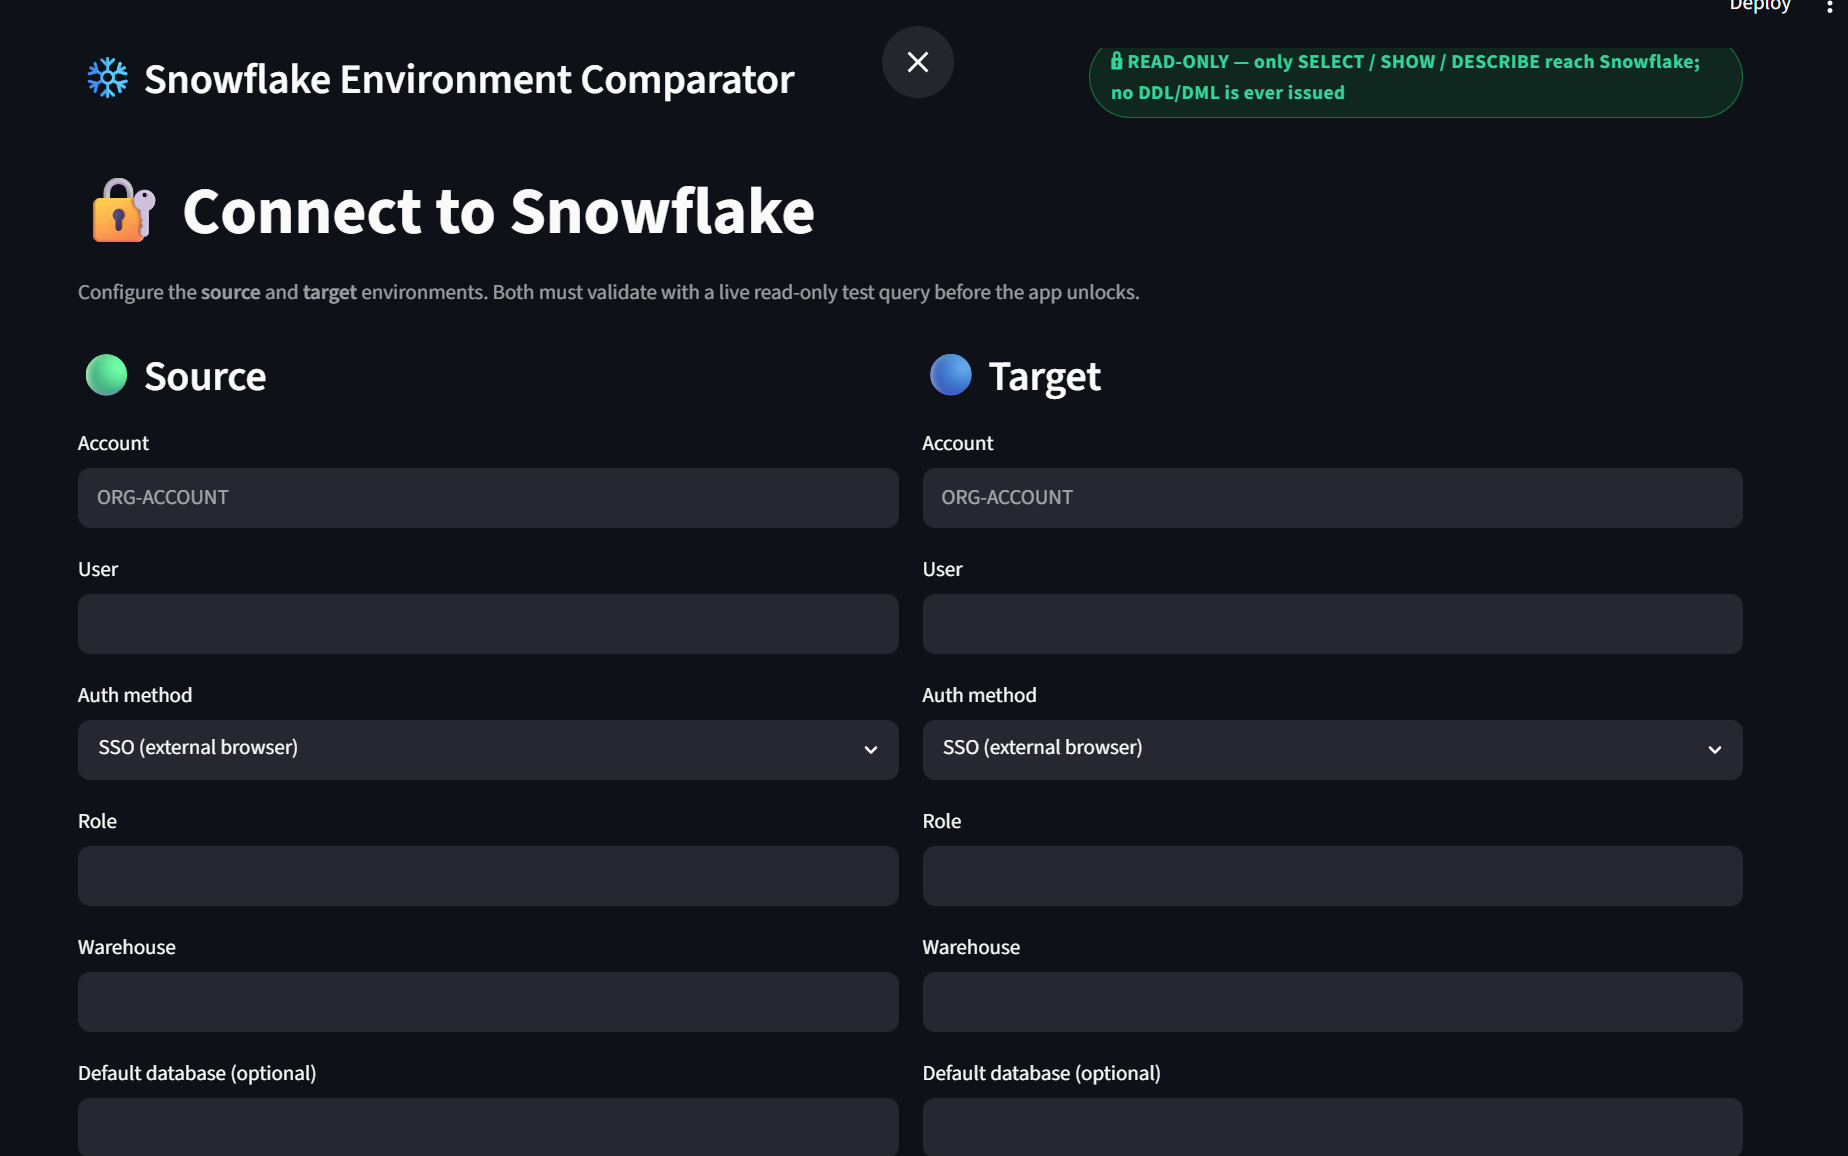
\includegraphics[width=\linewidth]{comparator_gate.png}
  \caption{The connection gate. The engineer configures the source and target environments side by side; both must validate with a live read-only test query before the application unlocks. The permanent read-only banner states that only \texttt{SELECT}, \texttt{SHOW}, and \texttt{DESCRIBE} statements reach Snowflake.}
  \label{fig:gate}
\end{figure}

Figure~\ref{fig:gate} shows the entry screen, which realises the connection-gate design of Chapter~3. The engineer enters, for both the \emph{source} and the \emph{target}, the account, user, authentication method, role, warehouse, and an optional default database. The authentication selector exposes the methods accepted by the Snowflake connector---single sign-on through an external browser, username and password, and password with multi-factor authentication---so that environments enforcing MFA, such as \texttt{DEV}, can be reached. No screen beyond this gate is reachable until both connections validate with a live test query, which eliminates the risk of mistaking an unreachable environment for one with missing objects. The green banner at the top right---``\textsc{read-only --- only SELECT / SHOW / DESCRIBE reach Snowflake; no DDL/DML is ever issued}''---is displayed permanently, making the tool's safety posture visible at every step.

\subsection{Configuring and Launching a Comparison}
\label{subsec:impl-run}

\begin{figure}[H]
  \centering
  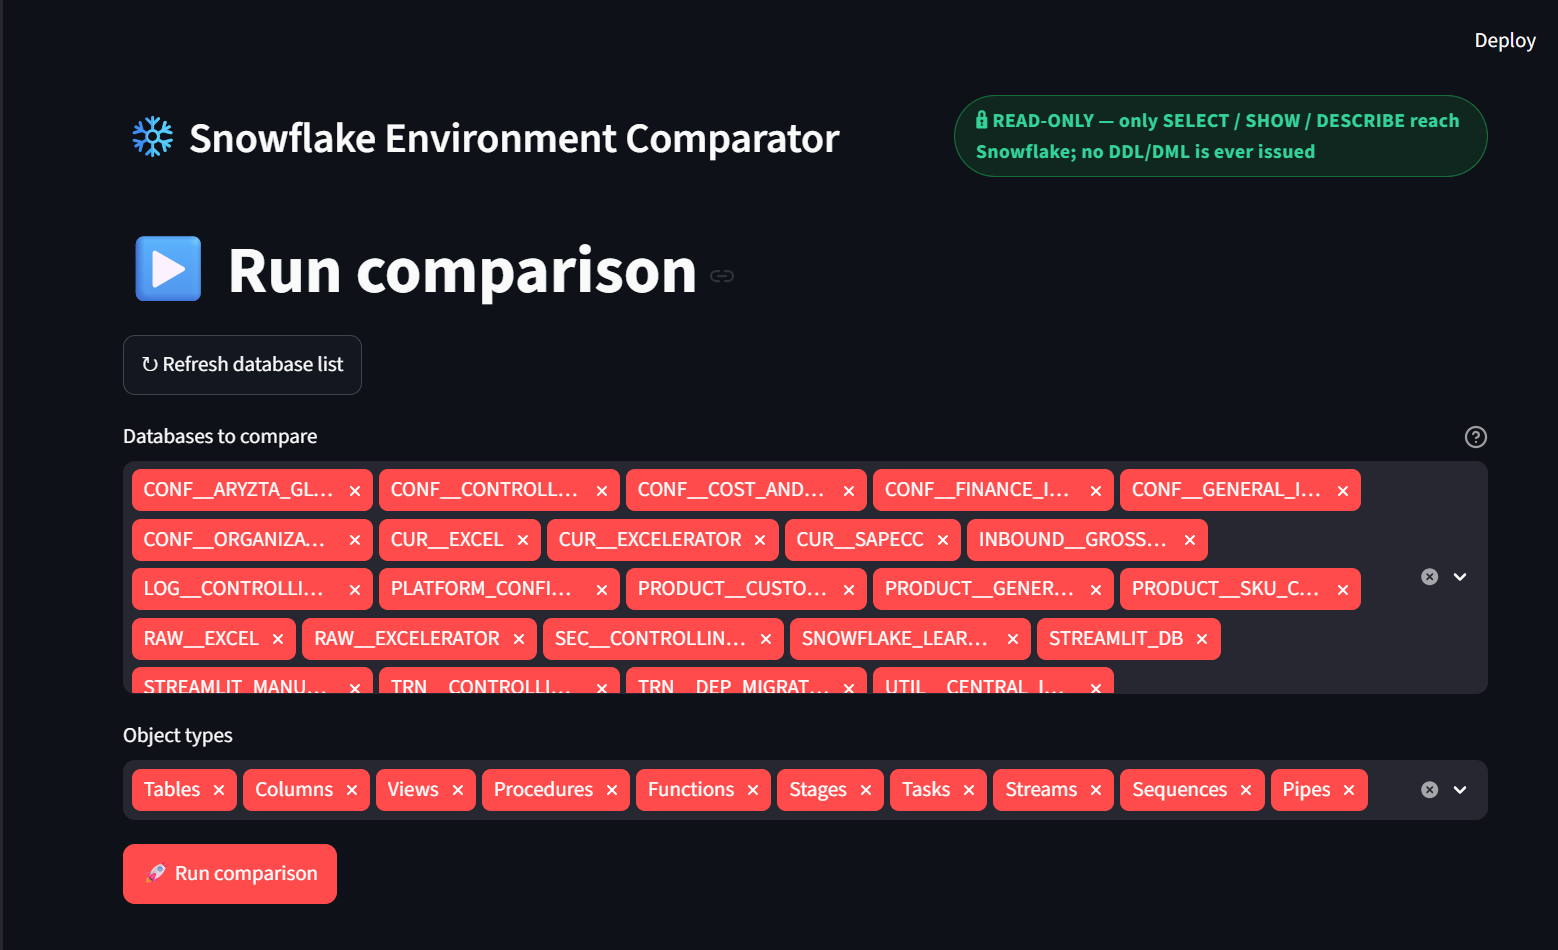
\includegraphics[width=\linewidth]{comparator_run.png}
  \caption{The run-configuration screen. The engineer selects the databases to compare and the object types to include, then launches the comparison. The database list is retrieved live from the connected accounts.}
  \label{fig:run}
\end{figure}

Once unlocked, the application presents the run-configuration screen of Figure~\ref{fig:run}. The engineer selects the databases to compare---retrieved live from the connected accounts and refreshable on demand---and the object types to include. All ten supported types are selectable: tables, columns, views, procedures, functions, stages, tasks, streams, sequences, and pipes. Launching the comparison triggers the ingestion-and-comparison process: the engine reads object metadata from both environments through the read-only reader, classifies every object, and persists the outcome.

\subsection{Comparison Results and Scorecard}
\label{subsec:impl-results}

\begin{figure}[H]
  \centering
  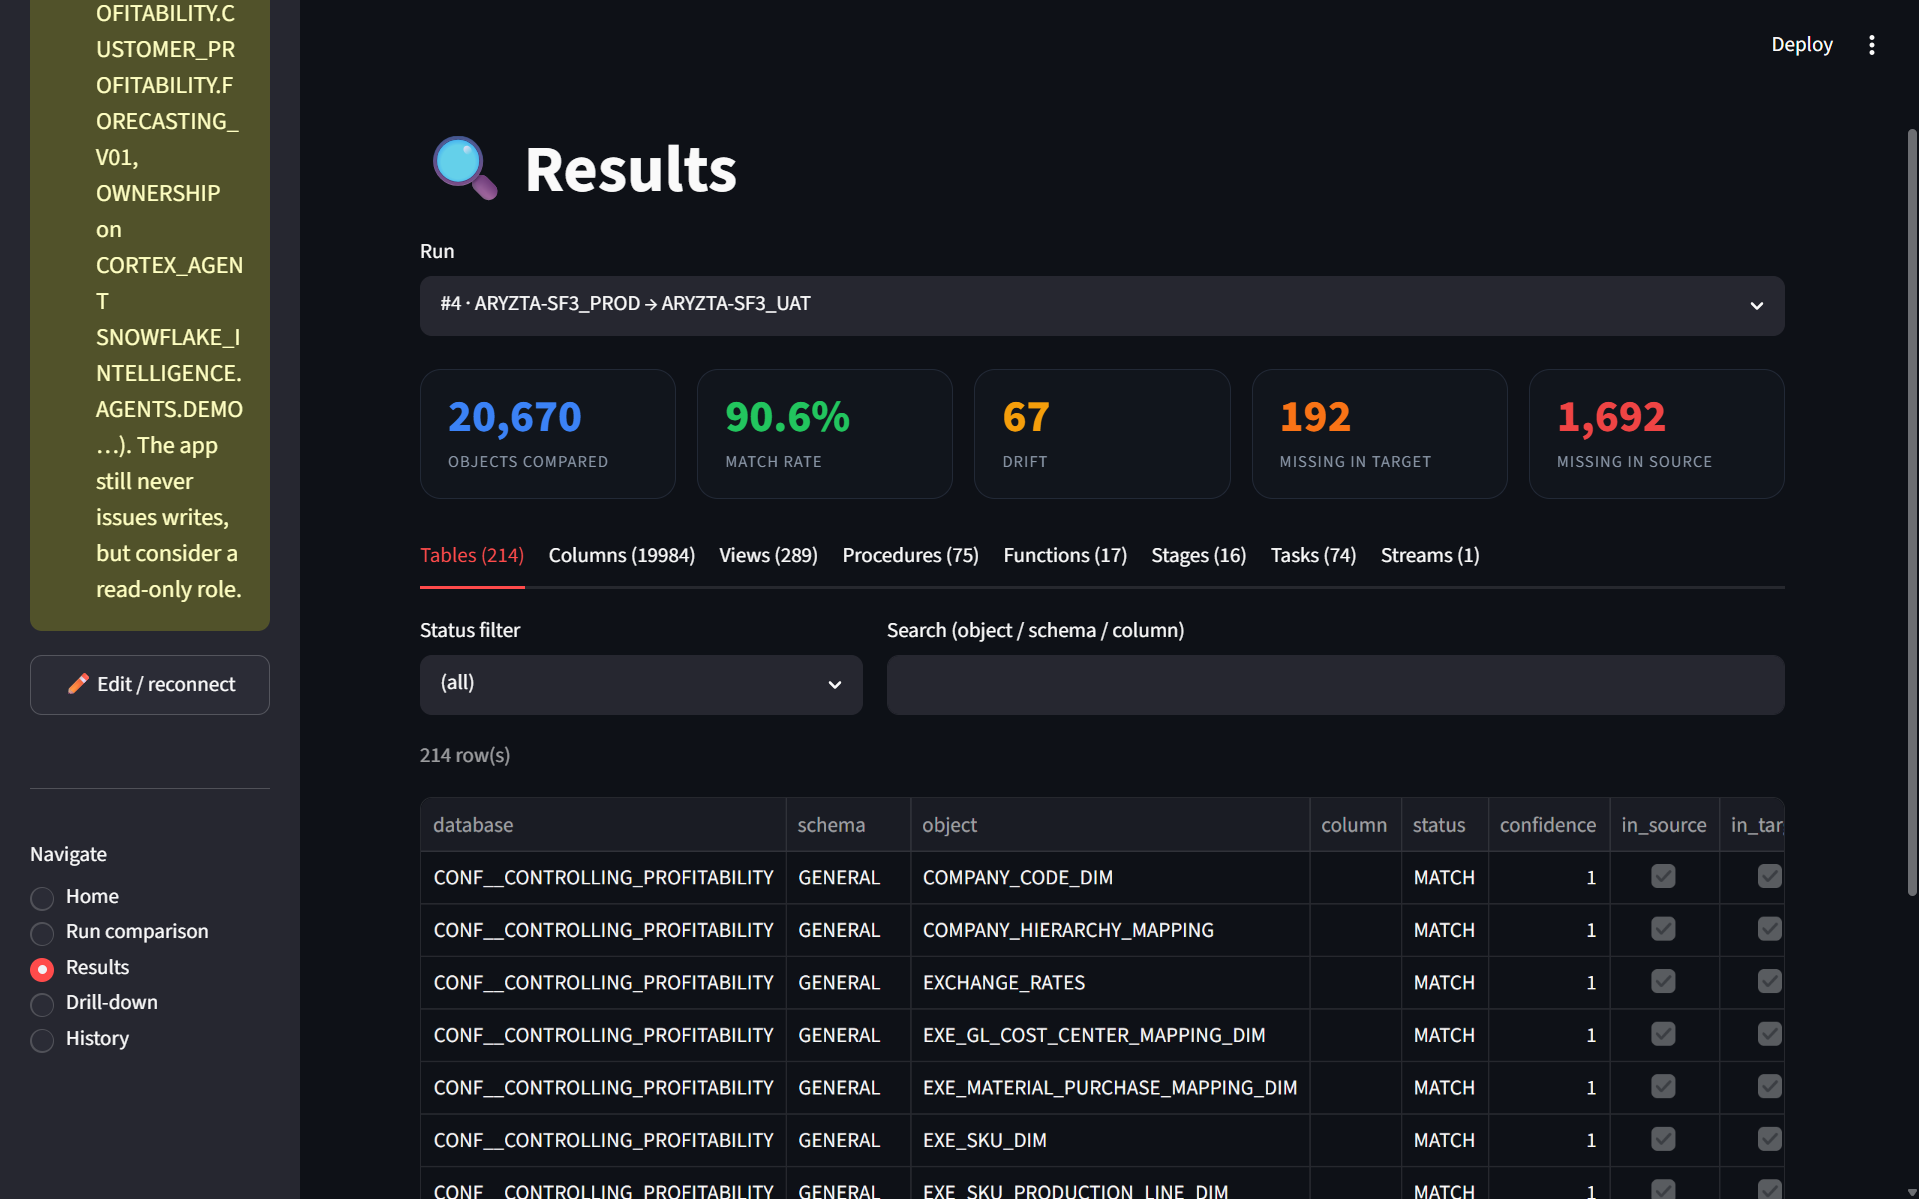
\includegraphics[width=\linewidth]{comparator_results.png}
  \caption{The results screen for a \texttt{PROD}-versus-\texttt{UAT} comparison. The scorecard reports the number of objects compared, the overall match rate, and the per-status tallies; the tabs break the results down by object type, and the table below supports filtering and search down to individual objects, columns, and attributes.}
  \label{fig:results}
\end{figure}

Figure~\ref{fig:results} presents the results screen, which is the principal output of the audit. The scorecard at the top quantifies the alignment of the selected environment pair: for the illustrated \texttt{PROD}-versus-\texttt{UAT} run, it reports \textbf{20{,}670 objects compared}, an overall \textbf{match rate of 90.6\%}, \textbf{67 drifted} objects, \textbf{192 missing in the target}, and \textbf{1{,}692 missing in the source}. The tabbed control beneath the scorecard breaks the figures down by object type---tables, columns, views, procedures, functions, stages, tasks, and streams---each annotated with its own count, while the searchable, filterable table at the bottom allows the engineer to drill down to an individual object, its status, its confidence score, and its presence on each side. This screen transforms the qualitative discrepancies described in Chapter~2 into precise, object-level measurements.

\subsection{Comparison History}
\label{subsec:impl-history}

\begin{figure}[H]
  \centering
  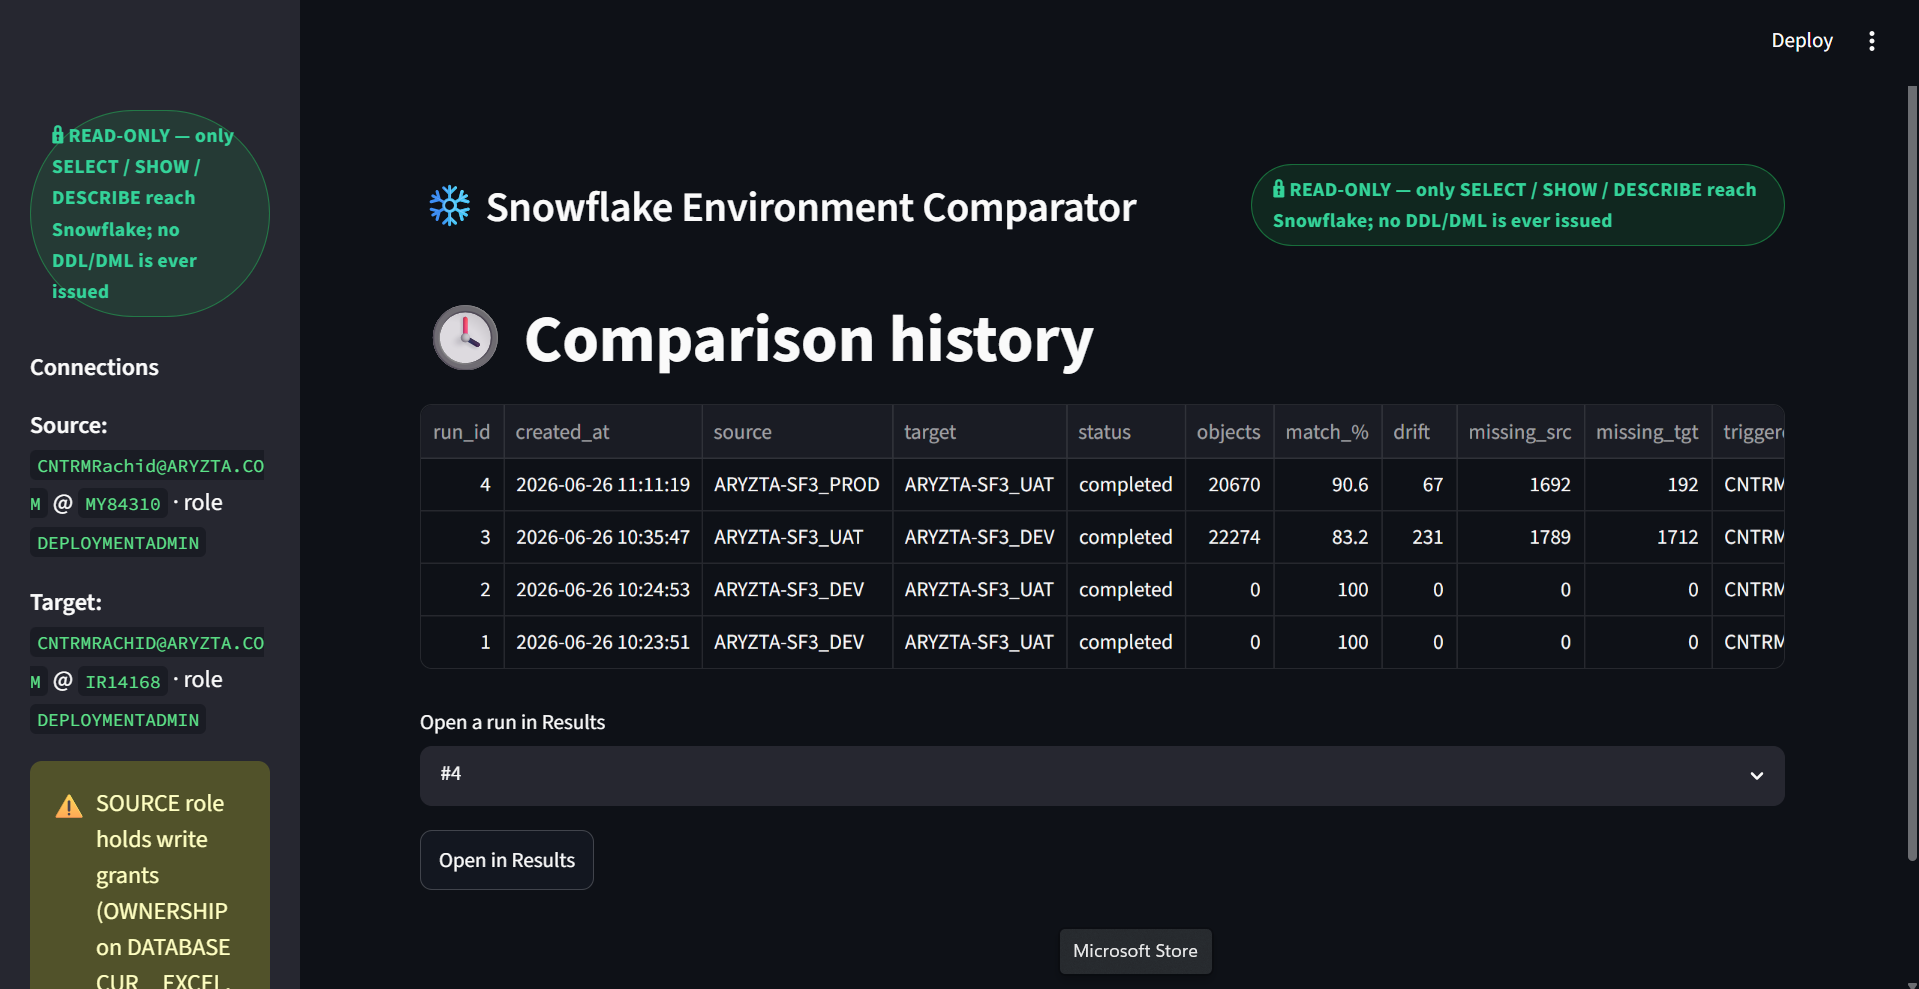
\includegraphics[width=\linewidth]{comparator_history.png}
  \caption{The comparison-history screen. Every run is persisted with its timestamp, source and target labels, status, and aggregate counts, and can be reopened in the results view.}
  \label{fig:history}
\end{figure}

Because every run is persisted to the SQLite store, the application retains a complete, queryable history, shown in Figure~\ref{fig:history}. Each entry records the run identifier, the timestamp, the source and target environments, the completion status, and the aggregate counts, and any past run can be reopened in the results view. This history is what gives the audit its durable, auditable character: the alignment of the environments can be re-measured at any time and the trajectory of the drift tracked across runs. The realisation of the comparator thus delivers not only a one-off diagnosis but a permanent instrument for monitoring the platform's health.

% ═══════════════════════════════════════════════════════════════
\section{Version Control and the CI/CD Pipeline}
\label{sec:impl-cicd}

The second workstream realises objectives O4 and O5: placing the Snowflake codebase under version control and automating its promotion across environments through a governed pipeline.

\subsection{Repository and Branching Model}
\label{subsec:impl-repo}

A GitHub repository (\texttt{aryzta-analytics-sf3}) was established as the authoritative source of truth for the platform's Snowflake objects and the deployment automation. The branching model maps each long-lived branch to one environment---\texttt{dev}~$\rightarrow$~\texttt{DEV}, \texttt{uat}~$\rightarrow$~\texttt{UAT}, and \texttt{main}~$\rightarrow$~\texttt{PROD}---and branch-protection rules require a reviewed pull request before any change can be merged into the upper-environment branches. This directly remedies the absence of code review and version control identified as root causes in Chapter~2: every change to the platform now has an author, a reviewer, and a permanent history.

\subsection{The End-to-End Deployment Workflow}
\label{subsec:impl-workflow}

\begin{figure}[H]
  \centering
  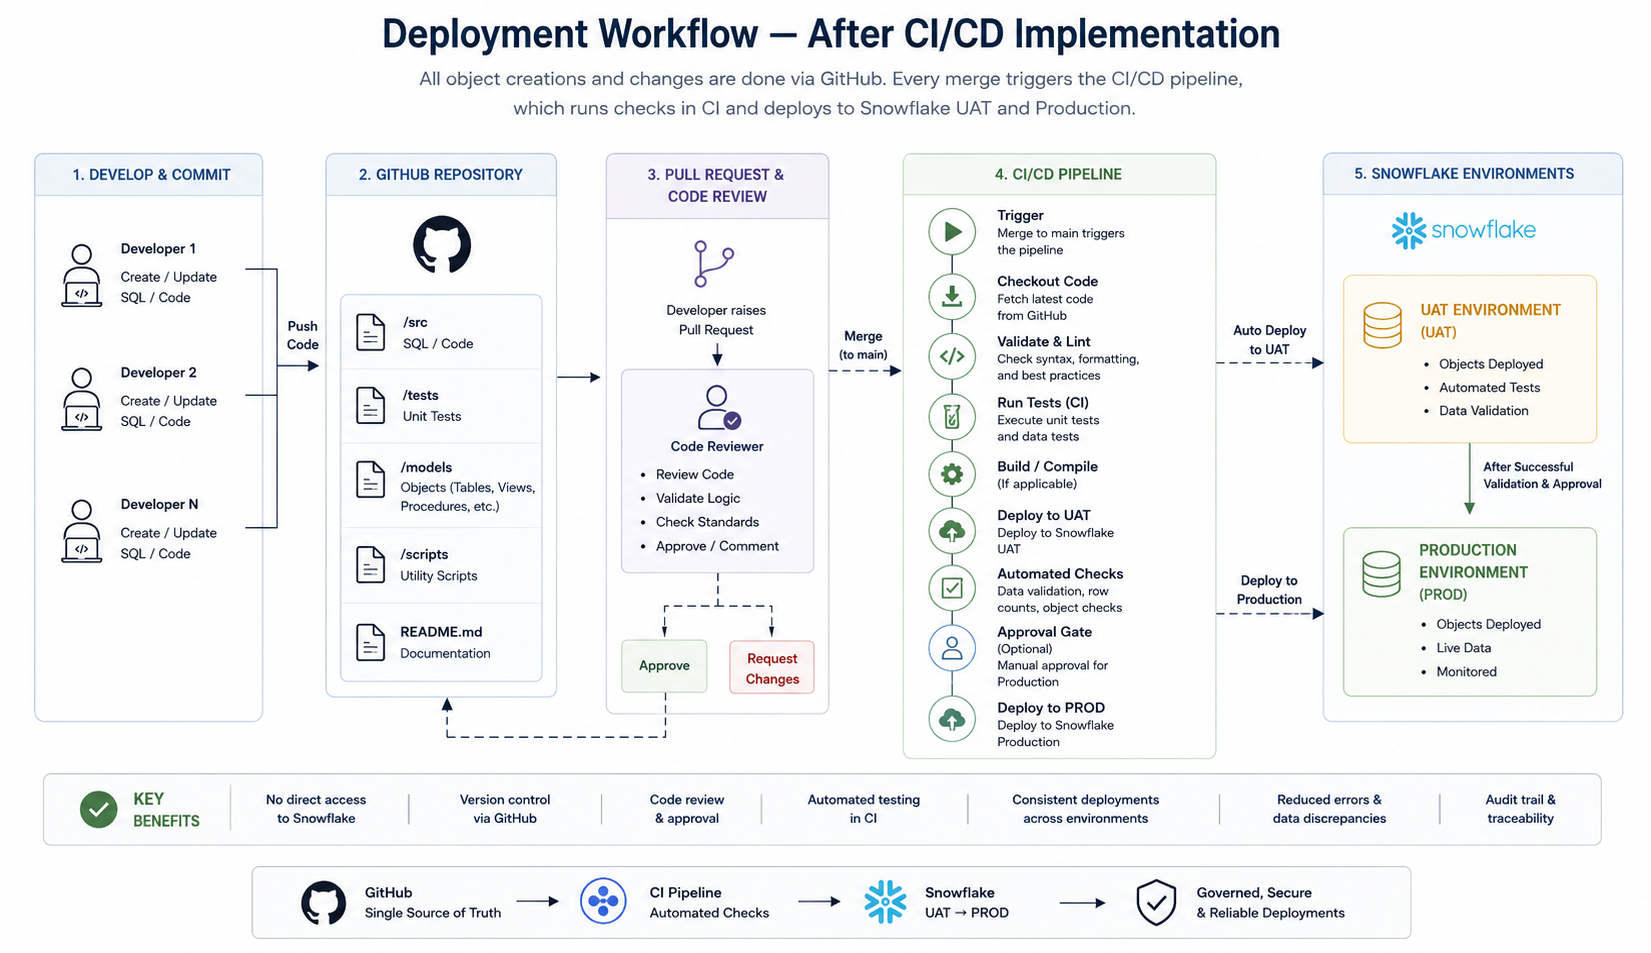
\includegraphics[width=\linewidth]{deployment_workflow.png}
  \caption{The deployment workflow after CI/CD implementation. A change flows from development and commit, through the GitHub repository and pull-request review, into the automated pipeline (checkout, validation, build, and staged deployment with an approval gate before production), and finally into the Snowflake environments.}
  \label{fig:deploy-workflow}
\end{figure}

Figure~\ref{fig:deploy-workflow} shows the governed path that every change now follows. A developer commits SQL changes to the repository; the change is reviewed through a pull request, where it can be approved or sent back for revision; once merged, the pipeline checks out the code, validates and lints it, and deploys it to \texttt{DEV} and then \texttt{UAT}; and only after a successful \texttt{UAT} stage and an explicit approval gate is the change deployed to \texttt{PROD}. The benefits annotated along the bottom of the diagram---a single source of truth, automated checks, governed deployments, reduced errors, and a complete audit trail---are precisely the properties whose absence Chapter~2 identified as the cause of the drift.

\subsection{GitHub Actions in Operation}
\label{subsec:impl-gh}

\begin{figure}[H]
  \centering
  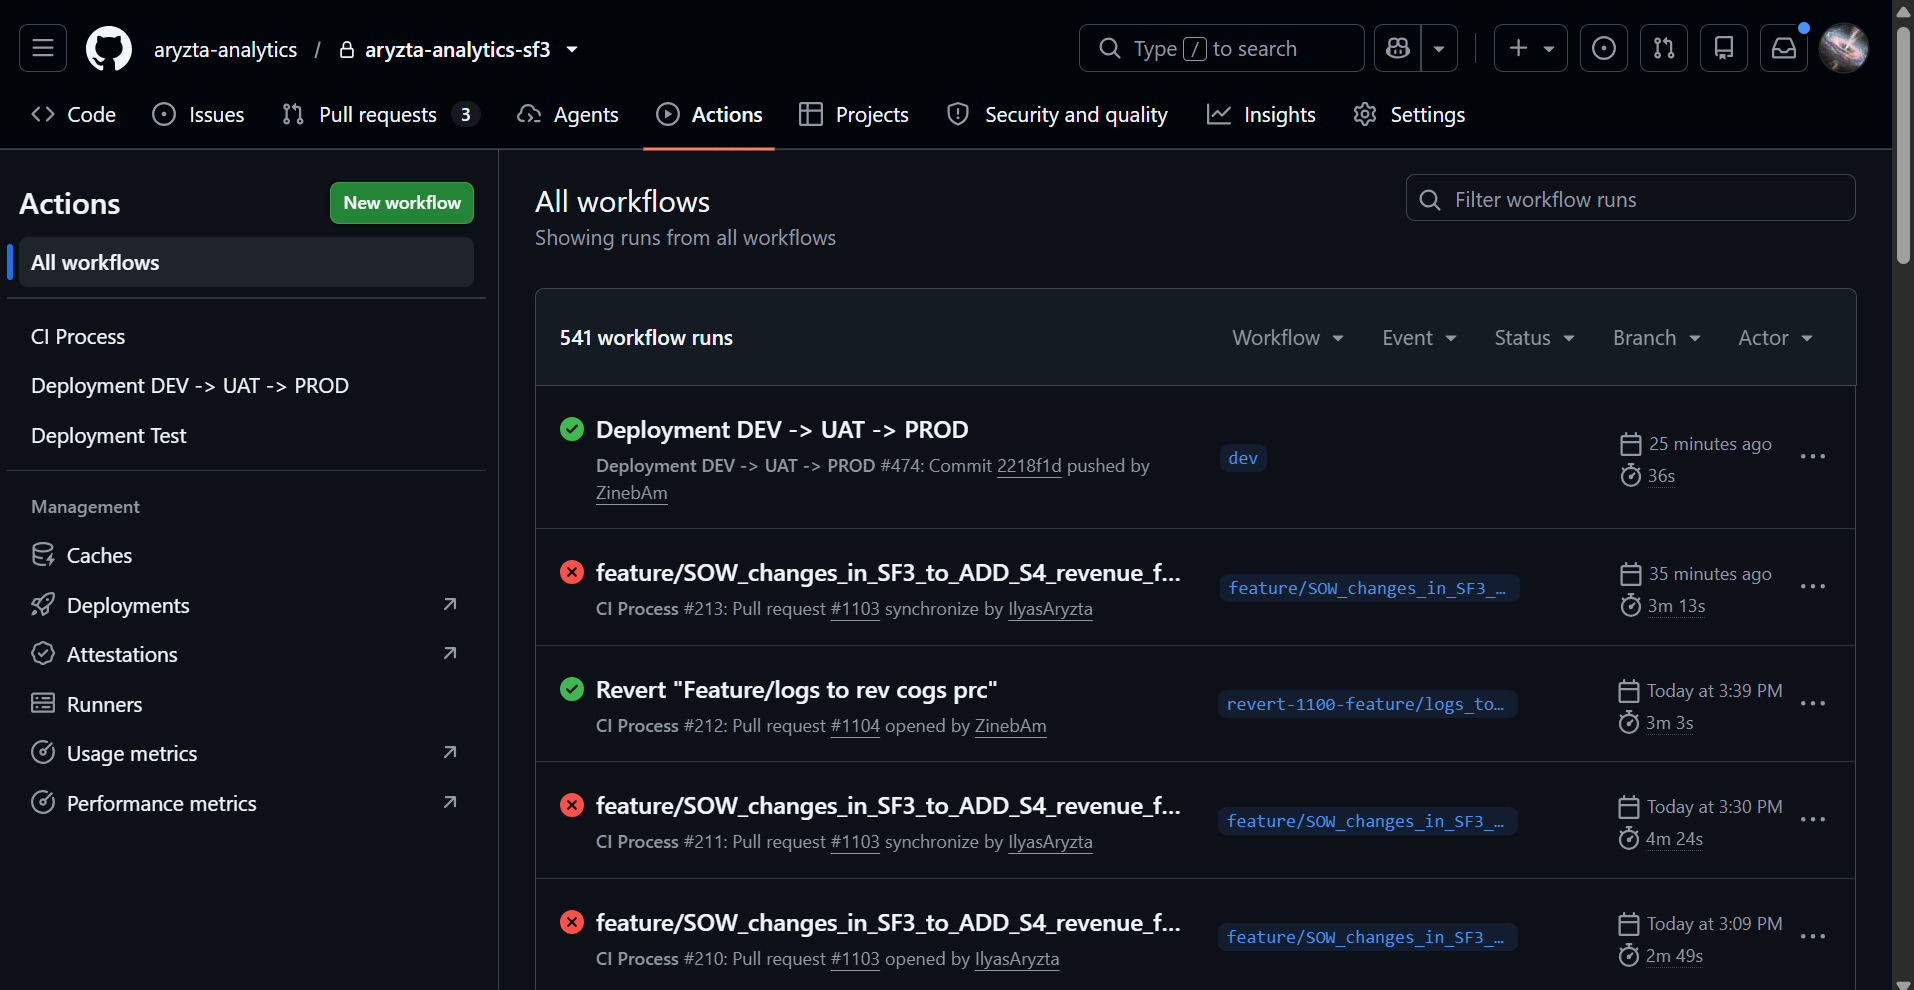
\includegraphics[width=\linewidth]{github_actions_home.png}
  \caption{The GitHub Actions view of the repository, showing the configured workflows---among them the \emph{Deployment DEV $\rightarrow$ UAT $\rightarrow$ PROD} pipeline---and the history of workflow runs triggered by commits and pull requests.}
  \label{fig:gh-home}
\end{figure}

The automation is implemented as GitHub Actions workflows, shown in operation in Figure~\ref{fig:gh-home}. The repository defines dedicated workflows---including a continuous-integration process and the \emph{Deployment DEV~$\rightarrow$~UAT~$\rightarrow$~PROD} pipeline---and the run history records hundreds of executions, each tied to a specific commit or pull request and to the engineer who initiated it. This run history is itself a governance artefact: it provides a complete, timestamped record of every deployment attempt and its outcome, the absence of which previously made incident analysis so difficult.

\begin{figure}[H]
  \centering
  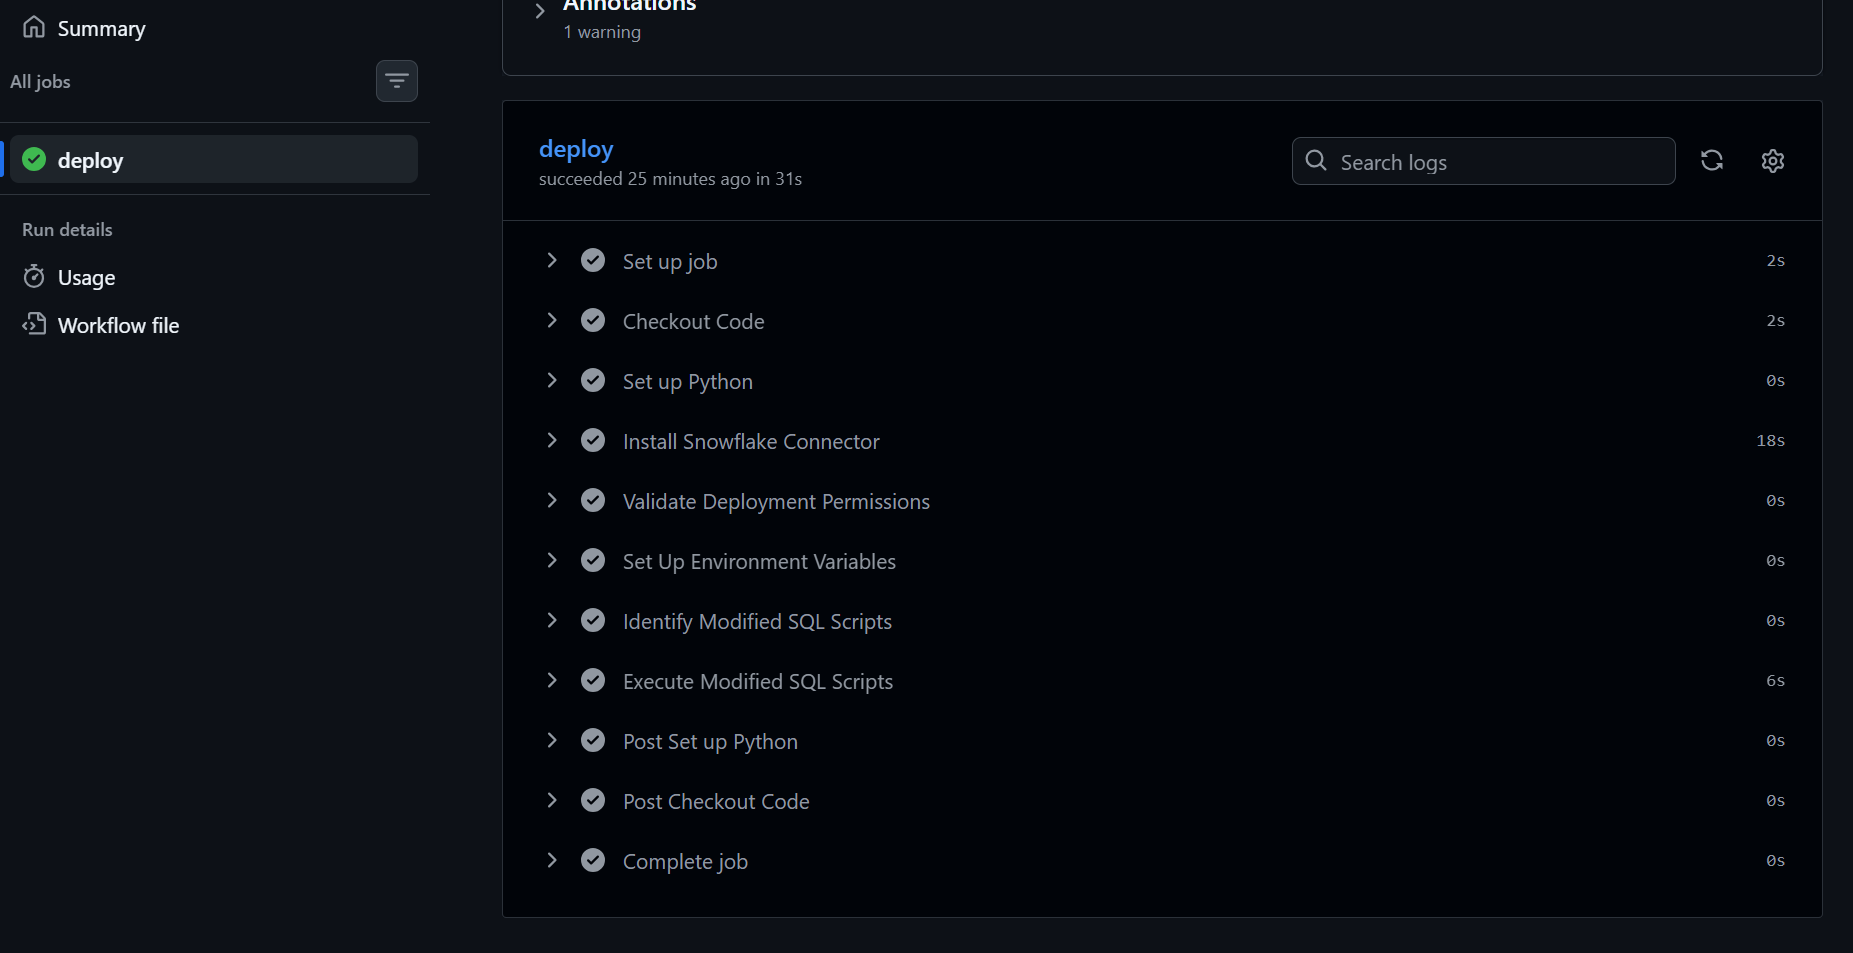
\includegraphics[width=\linewidth]{github_actions_deploy_job.png}
  \caption{A successful deployment job. The pipeline checks out the code, prepares the Python environment and the Snowflake connector, validates deployment permissions, identifies the modified SQL scripts, and executes them against the target environment.}
  \label{fig:gh-deploy}
\end{figure}

Figure~\ref{fig:gh-deploy} details a single deployment job. Its ordered steps---setting up the job, checking out the code, preparing Python, installing the Snowflake connector, \emph{validating deployment permissions}, setting up the environment variables, \emph{identifying the modified SQL scripts}, and \emph{executing} them---encode the deployment discipline that was previously absent. Two steps are particularly significant: the permission-validation step enforces that the pipeline deploys only with an authorised identity, and the change-detection step ensures that only the scripts actually modified by the change are applied, rather than a blanket re-execution. The job completes in seconds, illustrating that governance and speed are not in tension once the process is automated. For every promotion to \texttt{PROD}, the deployment is additionally associated with a ServiceNow change request, in line with ARYZTA's change-management policy described in Section~\ref{sec:project-mgmt}, establishing an auditable link between each production change and its authorising ticket.

% ═══════════════════════════════════════════════════════════════
\section{Deployment of the Synchronisation Solution}
\label{sec:impl-sync}

The third workstream deployed the share-based synchronisation designed in Section~\ref{sec:sync}, bringing \texttt{DEV} and \texttt{UAT} into ongoing alignment with \texttt{PROD}.

\subsection{Secure Data Shares}
\label{subsec:impl-shares}

\begin{figure}[H]
  \centering
  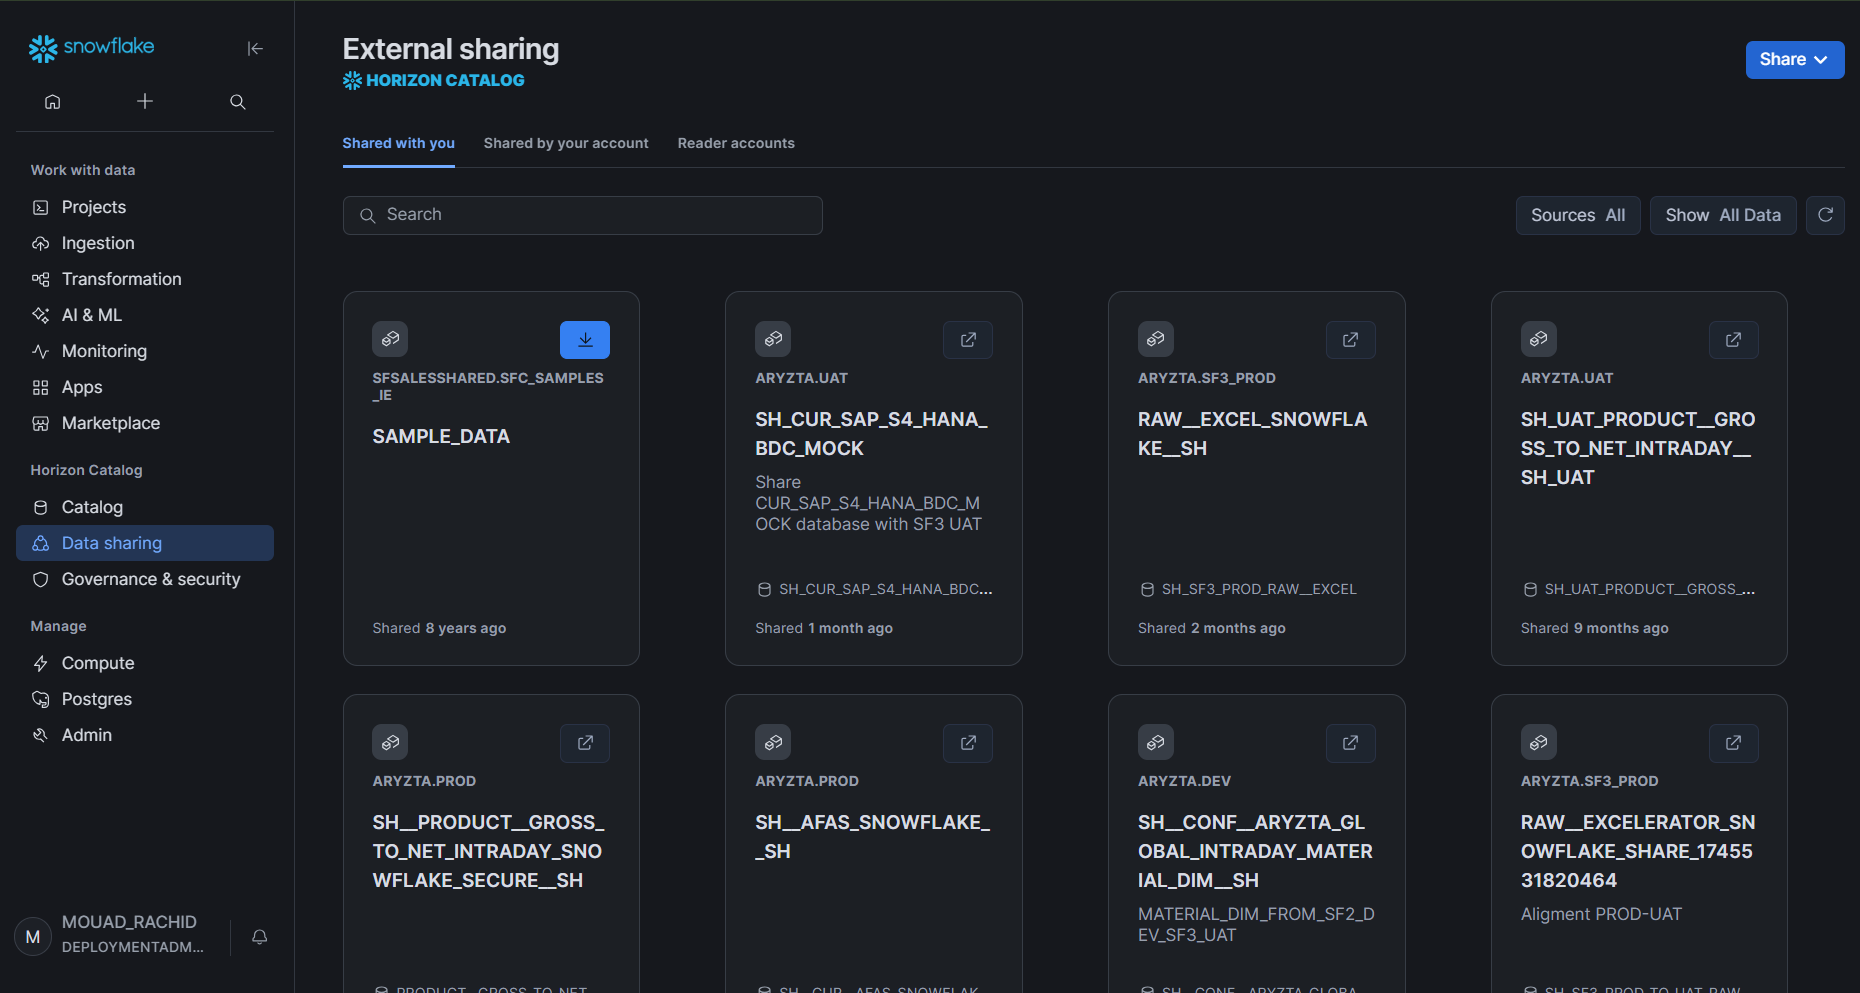
\includegraphics[width=\linewidth]{data_share.png}
  \caption{The inbound Secure Data Shares as seen from a consumer account. Each in-scope \texttt{PROD} database is exposed as a dedicated read-only share that the lower environments mount locally for synchronisation. (Share names are blurred for confidentiality.)}
  \label{fig:data-share}
\end{figure}

Figure~\ref{fig:data-share} shows the Secure Data Shares provisioned for the project, viewed from a consumer account's external-sharing catalogue (the individual share names are blurred for confidentiality). Each in-scope \texttt{PROD} database is published as its own read-only share, following the project's share-naming convention, and mounted as a local database in the \texttt{UAT} and \texttt{DEV} accounts. This realises the provider/consumer architecture of Chapter~3: production data is exposed live and read-only, without being copied, and remains the untouched source of truth.

\subsection{The Synchronisation Procedure in Operation}
\label{subsec:impl-sp}

\begin{figure}[H]
  \centering
  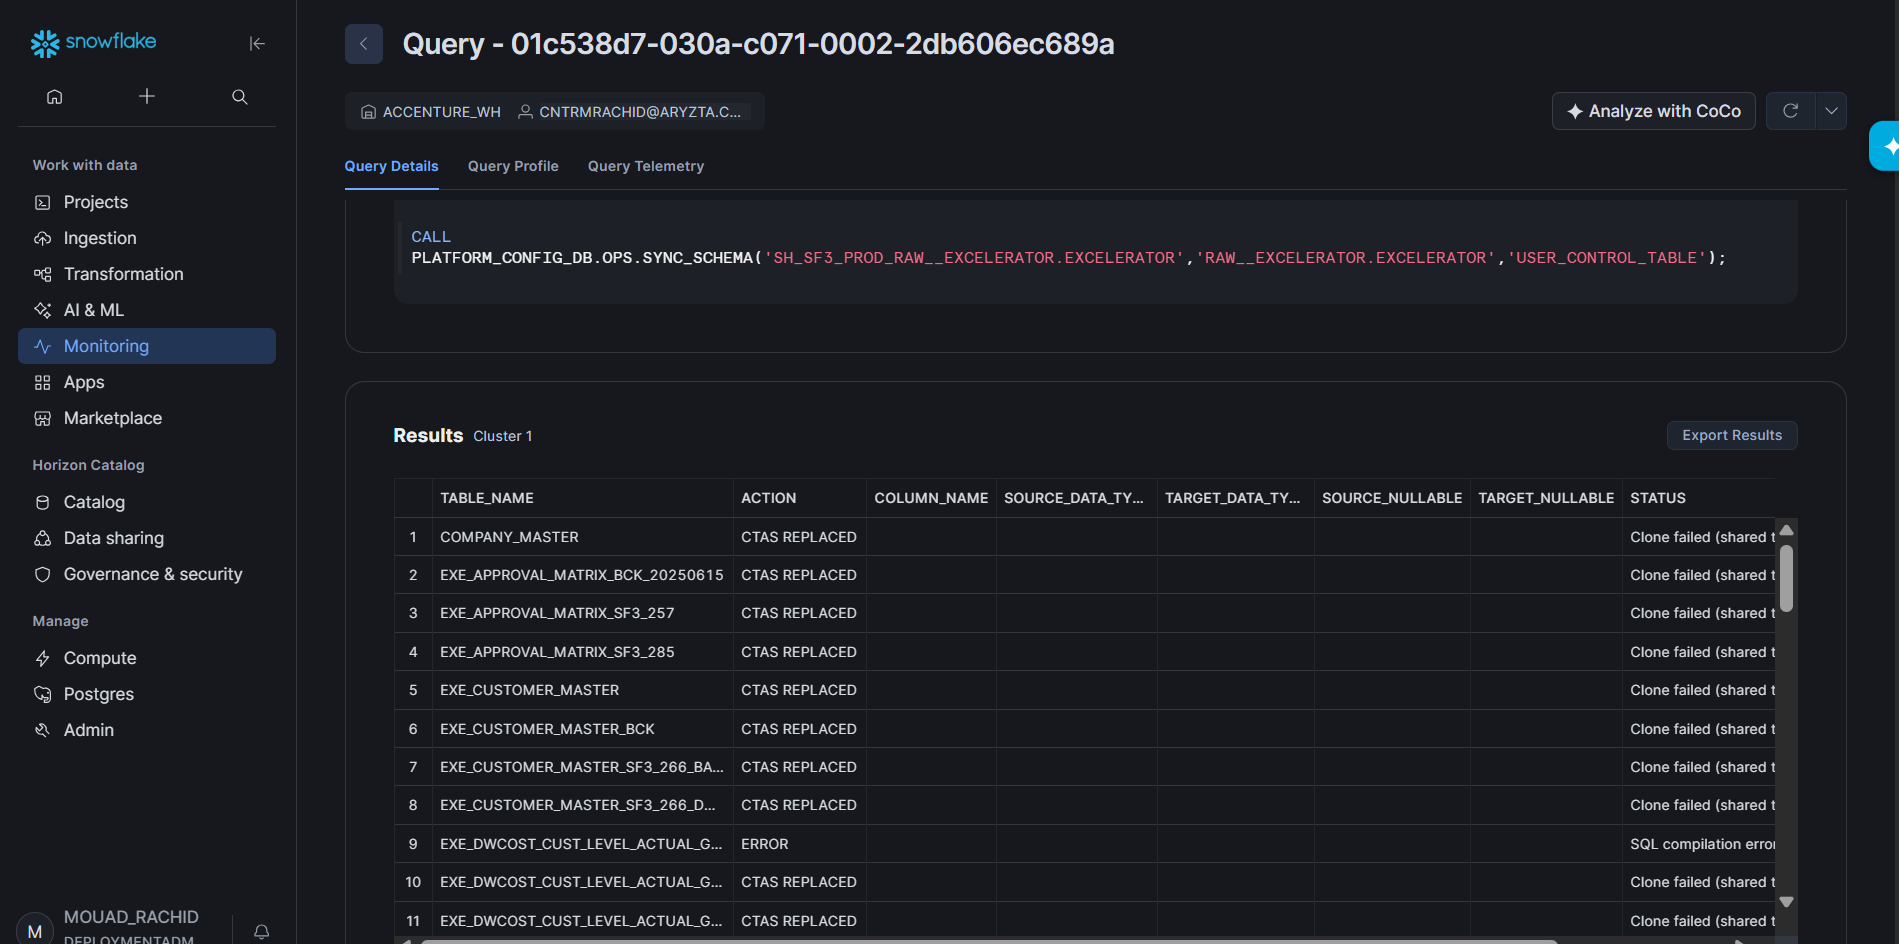
\includegraphics[width=\linewidth]{sync_procedure_run.png}
  \caption{A run of the synchronisation procedure in Snowflake. The procedure is invoked for a share-mounted source schema and a local target schema, and returns a log table recording, per table, the action taken and its outcome. (Database names are blurred for confidentiality.)}
  \label{fig:sync-run}
\end{figure}

Figure~\ref{fig:sync-run} shows the synchronisation procedure executing in Snowflake. The procedure is invoked for a given share-mounted source schema and local target schema, with a list of tables to exclude from the refresh. It returns a log table that records, for every table, the action taken and its result. In the illustrated run, many tables are refreshed via a create-table-as-select operation---the documented fallback for objects read from a share, where a direct clone is not permitted---each annotated accordingly in the log. This per-table log is the operational counterpart to the comparator's audit history: where the comparator measures drift on demand, the synchronisation log records, day by day, exactly which tables were refreshed and which exhibited structural divergence requiring a governed change through the pipeline.

\subsection{Daily Scheduling}
\label{subsec:impl-task}

The procedure is driven on a daily cadence by a Snowflake task in each consumer account. Because the procedure operates at schema granularity, the schedule invokes it once for each in-scope schema, passing the appropriate exclusion list so that operational control tables are preserved. The task therefore reduces the entire alignment workload to a single, repeatable, self-documenting daily operation, replacing what had previously been an undocumented and manual effort.

% ═══════════════════════════════════════════════════════════════
\section{Limitations}
\label{sec:impl-limitations}

While the implemented solution meets the objectives set out in Chapter~1, a candid account must also acknowledge the limits of the approach, several of which open directions for future work:

\begin{itemize}
  \item \textbf{Data-level synchronisation only.} The synchronisation refreshes data and clones missing tables, but it does not reconcile structurally divergent tables automatically; such cases are logged and must be resolved through a governed DDL change in the pipeline. This is a deliberate safety choice rather than an oversight, but it means that full structural convergence still depends on human-authored migrations.
  \item \textbf{Scope bounded by the main DAG.} Synchronisation covers the fourteen databases touched by the main task DAG. Objects outside that backbone are not synchronised, by design, so their alignment is not guaranteed.
  \item \textbf{Single-user, local audit tool.} The comparator is operated locally by one engineer rather than running as a shared, always-on service; scaling it to scheduled, multi-user operation would require further engineering.
  \item \textbf{Daily cadence.} The synchronisation runs once per day, so the lower environments reflect production as of the last run rather than in real time.
  \item \textbf{Dependence on Secure Data Sharing semantics.} Tables read through a share cannot be cloned directly and are refreshed via a create-table-as-select fallback; this is functionally correct but less efficient than a zero-copy clone for very large tables.
\end{itemize}

% ═══════════════════════════════════════════════════════════════
\section*{Chapter Conclusion}

This chapter has documented the realisation of the three workstreams that constitute the project's technical contribution, presented through the delivered interfaces rather than through source code. The Snowflake Environment Comparator was shown in operation across its connection gate, run configuration, results scorecard, and history, demonstrating a strictly read-only tool that turns environment drift into precise, persisted measurements. Version control and an automated \gls{cicd} pipeline were shown on GitHub, mapping protected branches to environments and routing every change through reviewed pull requests, validation, environment-scoped deployment, and an approval gate before production, with production changes linked to ServiceNow change requests. Finally, the synchronisation solution was shown through its Secure Data Shares and a live run of the synchronisation procedure, confirming the daily, non-destructive realignment of \texttt{DEV} and \texttt{UAT} with \texttt{PROD}. Together, and within the limitations noted above, these artefacts deliver the audit, synchronisation, pipeline, integration, and governance objectives defined in Chapter~1, transforming a previously ungoverned platform into a measurable, version-controlled, and continuously aligned data environment.

\newpage


% ═══════════════════════════════════════════════════════════════
%  General Conclusion
% ═══════════════════════════════════════════════════════════════
\chapter*{General Conclusion and Perspectives}
\addcontentsline{toc}{chapter}{General Conclusion and Perspectives}
\markboth{General Conclusion and Perspectives}{General Conclusion and Perspectives}

This end-of-studies internship, conducted at IBM Client Innovation Center Morocco in collaboration with Hakkoda, has addressed a concrete and consequential challenge in enterprise data engineering: the remediation of a critically misaligned multi-environment Snowflake data platform and the establishment of the DevOps and DataOps practices necessary to prevent the recurrence of such misalignment.

The work documented in this report spans the full arc of the project. Chapter 1 established the organizational and technical context, introducing the host organization, the client ARYZTA, and the specific technical problem of environment drift arising from years of ungoverned, manual deployments to the Snowflake production environment. Chapter 2 provided a rigorous analysis of the current platform state, quantifying the scope of discrepancies, characterizing their business impact, and identifying both the organizational and technical root causes that gave rise to them. Chapter 3 set out the design of the solution---a strictly read-only audit tool and a Secure Data Sharing--based synchronization strategy---and Chapter 4 documented their implementation alongside a GitHub-integrated CI/CD pipeline, before closing on the limitations of the approach.

The analysis confirmed that the central root causes---absence of version control, lack of a deployment governance framework, and the normalization of direct production deployments---are addressable through well-established engineering practices. The solution designed and implemented over the course of the project centers on a read-only comparator that makes environment drift measurable, a daily share-based synchronization that realigns the lower environments with production, and a GitHub-integrated CI/CD pipeline that enforces version-controlled, pull-request-based promotion of changes through the DEV-UAT-PROD lifecycle, supported by automated validation and a documented governance framework.

\vspace{0.4cm}
\noindent\textbf{Key Contributions of This Internship}

The internship has produced the following tangible contributions to the ARYZTA data platform:

\begin{itemize}
  \item A comprehensive environment audit documenting all discrepancies between DEV, UAT, and PROD across all Snowflake object types.
  \item A structured root cause analysis identifying the organizational and technical factors underlying the observed environment drift.
  \item A multi-environment synchronization strategy designed to restore alignment between the three Snowflake accounts.
  \item A CI/CD pipeline architecture integrating GitHub Actions with Snowflake, enforcing version-controlled deployments with automated validation gates.
  \item A deployment governance framework defining roles, responsibilities, and change management procedures for the platform.
\end{itemize}

\vspace{0.4cm}
\noindent\textbf{Perspectives for Future Work}

The work completed during this internship establishes a solid foundation for the continued evolution of the ARYZTA data platform. Several directions for future development merit consideration:

\begin{itemize}
  \item \textbf{Adoption of dbt for Transformation Management}: Integrating the data build tool (\gls{dbt}) into the CI/CD pipeline would provide additional benefits in terms of transformation testing, documentation generation, and lineage tracking.
  \item \textbf{Automated Environment Refresh}: Implementing a mechanism to periodically refresh DEV and UAT with anonymized subsets of PROD data would further strengthen the representativeness of the lower environments for testing purposes.
  \item \textbf{Data Quality Gates in the Pipeline}: Introducing automated data quality checks as pipeline stages---using frameworks such as Great Expectations or Snowflake's native data quality features---would provide an additional layer of validation before changes reach production.
  \item \textbf{Expanded RBAC Implementation}: Further refinement of Snowflake's role-based access control model, aligned with the principle of least privilege, would enhance the platform's security posture and governance compliance.
  \item \textbf{Cost Monitoring and Optimization}: As the platform stabilizes under the new governance framework, attention can be directed toward Snowflake credit consumption optimization, leveraging auto-scaling policies, clustering keys, and materialization strategies.
\end{itemize}

\vspace{0.4cm}

On a personal level, this internship has provided a formative introduction to enterprise data engineering in a multinational consulting environment. Working within the IBM and Hakkoda teams has exposed me to the realities of large-scale cloud data platform management, the importance of DevOps discipline in sustaining platform health, and the value of structured analytical thinking in diagnosing and addressing complex technical problems. The experience has confirmed my intention to pursue a career in Data Engineering and DataOps, with a particular focus on cloud-native data platform architecture.

\newpage


% ── Bibliography ───────────────────────────────────────────────
\bibliographystyle{plainnat}
\bibliography{bibliography}
\addcontentsline{toc}{chapter}{Bibliography}

% ── Appendices ─────────────────────────────────────────────────
\appendix
% ═══════════════════════════════════════════════════════════════
%  Appendices
% ═══════════════════════════════════════════════════════════════

\chapter{Glossary of Technical Terms}
\label{app:glossary}

\begin{longtable}{l p{10cm}}
  \toprule
  \rowcolor{ibmblue!15}
  \textbf{Term} & \textbf{Definition} \\
  \midrule
  \endfirsthead
  \toprule
  \rowcolor{ibmblue!15}
  \textbf{Term} & \textbf{Definition} \\
  \midrule
  \endhead
  \bottomrule
  \endfoot

  Environment Drift       & The progressive divergence of software environments from a common baseline, caused by changes applied to one environment without being applied to others. \\[6pt]
  CI/CD Pipeline          & An automated sequence of steps that validate, test, and deploy code changes from a version control system to one or more target environments. \\[6pt]
  Snowflake Task          & A Snowflake-native object that schedules the execution of a SQL statement or stored procedure at a defined interval or in response to a trigger condition. \\[6pt]
  Snowflake Stream        & A Snowflake-native object that tracks Data Manipulation Language (DML) changes (inserts, updates, deletes) to a source table, enabling Change Data Capture patterns. \\[6pt]
  GitHub Actions          & A CI/CD platform integrated into GitHub that enables the definition of automated workflows triggered by repository events such as push, pull request, or schedule. \\[6pt]
  Pull Request            & A request to merge a branch into another branch in a version control system, typically subject to review by one or more team members before the merge is approved. \\[6pt]
  IaC (Infra-as-Code)     & A practice in which the desired state of infrastructure components is declared in machine-readable configuration files and applied through automated tooling. \\[6pt]
  DataOps                 & A set of practices, processes, and technologies that combine data engineering with DevOps principles to improve the quality, speed, and reliability of data pipeline delivery. \\[6pt]
  RBAC                    & Role-Based Access Control; a security model in which permissions to perform operations are assigned to roles, and users are granted roles rather than individual permissions. \\[6pt]
  Idempotency             & The property of an operation that produces the same result regardless of how many times it is applied. Idempotent deployment scripts can be re-executed safely without unintended side effects. \\[6pt]
  Technical Debt          & The implied cost of rework caused by choosing an expedient solution now instead of a more robust approach that would take longer. \\
\end{longtable}


\end{document}
